% 注意事项:编译两次,以确保目录、页码完整显示

\def\allfiles{}

\documentclass[14pt,a4paper,UTF8,twoside]{article}

% Formatting Packages ——————————————————————————————————————
\usepackage{multicol}
\usepackage{multirow}
\usepackage{enumitem}
\usepackage{indentfirst}
\usepackage[toc]{multitoc}

% Math & Physics Packages ————————————————————————————
\usepackage{amsmath, amsthm, amsfonts, amssymb}
\usepackage{setspace}
\usepackage{physics}
\usepackage{cancel}
\usepackage{nicefrac}
\usepackage{unicode-math} % 允许数学公式使用特定字体

% Image-related Packages —————————————————————————————
\usepackage{float} % 浮动体环境
\usepackage{subcaption} % 子图包
\usepackage{graphics, graphicx}
\usepackage{tikz, tikz-qtree}
\usepackage{mdframed}
\usepackage{lmodern}
\usetikzlibrary{arrows.meta}
\usetikzlibrary{shapes.geometric, arrows}
\tikzstyle{startstop} = [rectangle, rounded corners, minimum width=3cm, minimum height=1cm,text centered, draw=black, fill=red!30]
\tikzstyle{process} = [rectangle, minimum width=3cm, minimum height=1cm, text centered, draw=black, fill=blue!30]
\tikzstyle{arrow} = [thick,->,>=stealth]

\usepackage{pgfplots}
\pgfplotsset{compat=1.18}
\usepackage{xcolor}
\usepackage{fourier-orns}
\usepackage{lipsum}

% Colour Palette ——————————————————————————————————————
\definecolor{merah}{HTML}{F4564E}
\definecolor{merahtua}{HTML}{89313E}
\definecolor{biru}{HTML}{60BBE5}
\definecolor{birutua}{HTML}{412F66}
\definecolor{hijau}{HTML}{59CC78}
\definecolor{hijautua}{HTML}{366D5B}
\definecolor{kuning}{HTML}{FFD56B}
\definecolor{jingga}{HTML}{FBA15F}
\definecolor{ungu}{HTML}{8C5FBF}
\definecolor{lavender}{HTML}{CBA5E8}
\definecolor{merjamb}{HTML}{FFB6E0}
\definecolor{mygray}{HTML}{E6E6E6}
\definecolor{mygreen}{rgb}{0,0.6,0}
\definecolor{mymauve}{rgb}{0.58,0,0.82}

% Theorems ————————————————————————————————————————————
\usepackage{tcolorbox}
\usepackage{changepage}
\tcbuselibrary{skins,breakable,theorems}

\newcounter{hitung}
\setcounter{hitung}{\thesection}

\makeatletter
	% Proof 证明如下
	\def\tcb@theo@widetitle#1#2#3{\hbox to \textwidth{\textsc{\large#1}\normalsize\space#3\hfil(#2)}}
	\tcbset{
		theorem style/theorem wide name and number/.code={ \let\tcb@theo@title=\tcb@theo@widetitle},
		proofbox/.style={skin=enhancedmiddle,breakable,parbox=false,boxrule=0mm,
			check odd page, toggle left and right, colframe=black!20!white!92!hijau,
			leftrule=8pt, rightrule=0mm, boxsep=0mm,arc=0mm, outer arc=0mm,
			left=3mm,right=3mm,top=0mm,bottom=0mm, toptitle=0mm,
			bottomtitle=0mm,colback=gray!3!white!98!biru, before skip=8pt, after skip=8pt,
			before={\par\vskip-2pt},after={\par\smallbreak},
		},
	}
	\newtcolorbox{ProofBox}{proofbox}
	\makeatother
	
	\let\realproof\proof
	\let\realendproof\endproof
	\renewenvironment{proof}[1][Thoughts:]{\ProofBox\strut\textsc{#1}\space}{\endProofBox}
        \AtEndEnvironment{proof}{\null\hfill$\blacksquare$}
        % Definition 定义环境
	\newtcbtheorem[use counter=hitung, number within=section]{dfn}{定义}
	{theorem style=theorem wide name and number,breakable,enhanced,arc=3.5mm,outer arc=3.5mm,
		boxrule=0pt,toprule=1pt,leftrule=0pt,bottomrule=1pt, rightrule=0pt,left=0.2cm,right=0.2cm,
		titlerule=0.5em,toptitle=0.1cm,bottomtitle=-0.1cm,top=0.2cm,
		colframe=white!10!biru,
		colback=white!90!biru,
		coltitle=white,
		shadow={1.3mm}{-1.3mm}{0mm}{gray!50!white}, % 添加阴影
        coltext=birutua!60!gray, title style={white!10!biru}, rbefoe skip=8pt, after skip=8pt,
		fonttitle=\bfseries,fontupper=\normalsize}{dfn}

	% 答题卡
	\newtcbtheorem[use counter=hitung, number within=section]{ans}{解答}
	{theorem style=theorem wide name and number,breakable,enhanced,arc=3.5mm,outer arc=3.5mm,
		boxrule=0pt,toprule=1pt,leftrule=0pt,bottomrule=1pt, rightrule=0pt,left=0.2cm,right=0.2cm,
		titlerule=0.5em,toptitle=0.1cm,bottomtitle=-0.1cm,top=0.2cm,
		colframe=white!10!biru,
		colback=white!90!biru,
		coltitle=white,
		shadow={1.3mm}{-1.3mm}{0mm}{gray!50!white}, % 添加阴影
        coltext=birutua!60!gray, title style={white!10!biru}, before skip=8pt, after skip=8pt,
		fonttitle=\bfseries,fontupper=\normalsize}{ans}

	% Axiom
	\newtcbtheorem[use counter=hitung, number within=section]{axm}{公理}
	{theorem style=theorem wide name and number,breakable,enhanced,arc=3.5mm,outer arc=3.5mm,
		boxrule=0pt,toprule=1pt,leftrule=0pt,bottomrule=1pt, rightrule=0pt,left=0.2cm,right=0.2cm,
		titlerule=0.5em,toptitle=0.1cm,bottomtitle=-0.1cm,top=0.2cm,
		colframe=white!10!biru,colback=white!90!biru,coltitle=white,
		shadow={1.3mm}{-1.3mm}{0mm}{gray!50!white!90}, % 添加阴影
        coltext=birutua!60!gray,title style={white!10!biru},before skip=8pt, after skip=8pt,
		fonttitle=\bfseries,fontupper=\normalsize}{axm}
 
	% Theorem
	\newtcbtheorem[use counter=hitung, number within=section]{thm}{Warning}
	{theorem style=theorem wide name and number,breakable,enhanced,arc=3.5mm,outer arc=3.5mm,
		boxrule=0pt,toprule=1pt,leftrule=0pt,bottomrule=1pt, rightrule=0pt,left=0.2cm,right=0.2cm,
		titlerule=0.5em,toptitle=0.1cm,bottomtitle=-0.1cm,top=0.2cm,
		colframe=white!10!merah,colback=white!75!pink,coltitle=white, coltext=merahtua!80!merah,
		shadow={1.3mm}{-1.3mm}{0mm}{gray!50!white!90}, % 添加阴影
		title style={white!10!merah}, before skip=8pt, after skip=8pt,
		fonttitle=\bfseries,fontupper=\normalsize}{thm}
	
	% Proposition
	\newtcbtheorem[use counter=hitung, number within=section]{prp}{命题}
	{theorem style=theorem wide name and number,breakable,enhanced,arc=3.5mm,outer arc=3.5mm,
		boxrule=0pt,toprule=1pt,leftrule=0pt,bottomrule=1pt, rightrule=0pt,left=0.2cm,right=0.2cm,
		titlerule=0.5em,toptitle=0.1cm,bottomtitle=-0.1cm,top=0.2cm,
		colframe=white!10!hijau,colback=white!90!hijau,coltitle=white, coltext=hijautua!80!brown,
		shadow={1.3mm}{-1.3mm}{0mm}{gray!50!white}, % 添加阴影
		title style={white!10!hijau}, before skip=8pt, after skip=8pt,
		fonttitle=\bfseries,fontupper=\normalsize}{prp}


	% Example
	\newtcolorbox[use counter=hitung, number within=section]{cth}[1][]{breakable,
		colframe=white!10!jingga, coltitle=white!90!jingga, colback=white!85!jingga, coltext=black!10!brown!50!jingga, colbacktitle=white!10!jingga, enhanced, fonttitle=\bfseries,fontupper=\normalsize, attach boxed title to top left={yshift=-2mm}, before skip=8pt, after skip=8pt,
		title=Tips~\thetcbcounter \ \ #1}

	% Catatan/Note
	\newtcolorbox{ctt}[1][]{enhanced, 
		left=4.1mm, borderline west={8pt}{0pt}{white!10!kuning}, 
		before skip=6pt, after skip=6pt, 
		colback=white!85!kuning, colframe= white!85!kuning, coltitle=orange!60!kuning!25!brown, coltext=orange!60!kuning!25!brown,
		fonttitle=\bfseries,fontupper=\normalsize, before skip=8pt, after skip=8pt,
		title=\underline{Notice}  #1}
	
	% Komentar/Remark
	\newtcolorbox{rmr}[1][]{
		,arc=0mm,outer arc=0mm,
		boxrule=0pt,toprule=1pt,leftrule=0pt,bottomrule=5pt, rightrule=0pt,left=0.2cm,right=0.2cm,
		titlerule=0.5em,toptitle=0.1cm,bottomtitle=-0.1cm,top=0.2cm,
		colframe=white!10!kuning,colback=white!85!kuning,coltitle=white, coltext=orange!60!kuning,
		fonttitle=\bfseries,fontupper=\normalsize, before skip=8pt, after skip=8pt,
		title=Remark#1}

\usepackage{booktabs} % 表格库
\usepackage{titlesec} % 标题库
\usepackage{fancyhdr} % 页眉页脚库
\usepackage[sorting=none]{biblatex}
\usepackage{array}
\usepackage{longtable}
\usetikzlibrary{positioning, arrows.meta}
\addbibresource{references.bib} % 指定你的.bib文件名称

\date{} % 留空,以让编译时去除日期

%———————————————注意事项—————————————————%

% 1、如果编译显示失败,但没有错误信息,就是 filename.pdf 正在被占用
% 2、在文件夹中的终端使用 Windows > xelatex filename.tex 也可编译

%—————————————华东师范大学———————————————%

% 论文制作时须加页眉,页眉从中文摘要开始至论文末
% 偶数页码内容为:华东师范大学硕士学位论文,奇数页码内容为学位论文题目

%————————定义 \section 的标题样式————————%

% 注意:\chapter 等命令,内部使用的是 \thispagestyle{plain} 的排版格式
% 若需要自己加上页眉,实际是在用 \thispagestyle{fancy} 的排版格式
% 加上下面这一段指令,就能够让 \section 也使用 fancy 的排版格式
% 本质就是让目录、第一页也能够显示页眉、页脚

\fancypagestyle{plain}{
  \pagestyle{fancy}
}

\title{华东师范大学软件学院实验报告} % 模板
\titleformat{\section}
    {\normalfont\bfseries\Large} % 字体大小、字体系列(\bfseries 为加粗)
    {\thesection}{1em}{}

% ———————————设置章节的中文格式———————————%
\renewcommand\thesection{\chinese{section} \hspace{0pt}}
\renewcommand\thesubsection{\arabic{subsection} \hspace{0pt}}
% \renewcommand\thesubsubsection{\alph{subsubsection} \hspace{0pt}} % 字母编号
% \hspace{0pt} 是为了确保在章节编号和章节题目之间不要有空格,使得排版更为美观
    
%—————————————页面基础设置———————————————%

\usepackage{geometry}
\geometry{left=10mm, right=10mm, top=20mm, bottom=20mm}

%————————————设置页眉、页脚——————————————%

\pagestyle{fancy} % 设置 plain style 的属性

% 设置页眉

\fancyhead[RE]{\footnotesize \leftmark} % Right Even 偶数页右侧显示章名 \leftmark 最高级别章名
\fancyhead[LO]{\footnotesize \rightmark} % Left Odd 奇数页左侧显示节名 \rightmark 第二级别节名
\fancyhead[C]{华东师范大学软件学院实验报告} % Center 居中显示
\fancyhead[LE,RO]{~\thepage~} % 在偶数页的左侧,奇数页的右侧显示页码
\renewcommand{\headrulewidth}{1.2pt} % 页眉与正文之间的水平线粗细

% 设置页脚:在每页的右下脚以斜体显示书名

\fancyfoot[RO,RE]{\it Lab Report By \LaTeX} % 使用意大利斜体显示
\renewcommand{\footrulewidth}{0.5pt} % 页脚水平线宽度

%——————设置页码:在底部居中显示页码———————%

\usepackage{lastpage} % 页码数库
\pagestyle{fancy}
\fancyfoot[C]{\kaishu 第 \thepage 页 \ 共 \pageref{LastPage} 页} % LastPage 需要二次编译以获取总页数

%——————————————代码块设置———————————————%

\usepackage{listings} % 代码块包
\lstset {
    backgroundcolor=\color{white},   % choose the background color; you must add \usepackage{color} or \usepackage{xcolor}
    basicstyle=\footnotesize,        % the size of the fonts that are used for the code
    breakatwhitespace=false,         % sets if automatic breaks should only happen at whitespace
    breaklines=true,                 % sets automatic line breaking
    captionpos=bl,                   % sets the caption-position to bottom
    commentstyle=\color{mygreen},    % comment style
    deletekeywords={...},            % if you want to delete keywords from the given language
    escapeinside={\%*}{*},           % if you want to add LaTeX within your code
    extendedchars=true,              % lets you use non-ASCII characters; for 8-bits encodings only, does not work with UTF-8
    frame=single,                    % adds a frame around the code
    keepspaces=true,                 % keeps spaces in text, useful for keeping indentation of code (possibly needs columns=flexible)
    keywordstyle=\color{blue},       % keyword style
    % language=Python,               % the language of the code
    morekeywords={*,...},            % if you want to add more keywords to the set
    numbers=left,                    % where to put the line-numbers; possible values are (none, left, right)
    numbersep=5pt,                   % how far the line-numbers are from the code
    numberstyle=\tiny\color{mygray}, % the style that is used for the line-numbers
    rulecolor=\color{black},         % if not set, the frame-color may be changed on line-breaks within not-black text (e.g. comments (green here))
    showspaces=false,                % show spaces everywhere adding particular underscores; it overrides 'showstringspaces'
    showstringspaces=false,          % underline spaces within strings only
    showtabs=false,                  % show tabs within strings adding particular underscores
    stepnumber=1,                    % the step between two line-numbers. If it's 1, each line will be numbered
    stringstyle=\color{orange},      % string literal style
    tabsize=2,                       % sets default tabsize to 2 spaces
    % title=Python Code              % show the filename of files included with \lstinputlisting; also try caption instead of title
}

% 注释掉的部分用于后续插入代码,参数可调整,格式如下:

% 1、直接插入
% \begin{lstlisting}[language = ? , title = { ? } ]
%       Your code here.
% \end{lstlisting}

% 2、文件插入
% \lstinputlisting[language = C , title = ?.c] {filename.c}

%———————————————字体设置————————————————%

\usepackage{fontspec} % 允许设置字体
\usepackage[utf8]{inputenc}
\usepackage{ctex}
\usepackage{pifont}
\linespread{1.2}
% \setCJKmainfont{SimSun} % 设置正文罗马族的 CJK 字体
\renewcommand{\texttt}[1]{\textcolor{blue}{\ttfamily #1}}

%———————————————超链接设置——————————————%

\usepackage[hidelinks]{hyperref}
\hypersetup{
    pdfstartview=FitH, % 设置PDF文档打开时的初始视图为页面宽度适应窗口宽度(即页面水平适应)
    CJKbookmarks=true, % 用对CJK(中文、日文、韩文)字符的书签支持,确保这些字符在书签中正确显示
    bookmarksnumbered=true, % 书签带有章节编号。这对有章节编号的文档很有用
    bookmarksopen=true, % 文档打开时,书签树是展开的,方便查看所有书签
    colorlinks, % 启用彩色链接。这样,链接在PDF中会显示为彩色,而不是默认的方框
    pdfborder=001, % 设置PDF文档中链接的边框样式。001 表示链接周围没有边框,仅在单击时显示一个矩形
    linkcolor=blue, % 设置文档内部链接(如目录中的章节链接)的颜色为蓝色
    anchorcolor=blue, % 设置锚点链接(即目标在同一文档内的链接)的颜色为蓝色
    citecolor=blue, % 设置引用(如文献引用)的颜色为蓝色
}

%————————————导言区结束,进入正文部分————————————%

\begin{document}

\maketitle

\begin{center} % \extracolsep{\fill} 拉伸到页面最大宽度前,保证居中显示

    \begin{tabular*}{\textwidth}{@{\extracolsep{\fill}} l  l  l }
        \hline
        课程名称:操作系统 &  年级:2023级本科  &  上机实践成绩:\ \ \ \ \ \ \ \ \ \ \ \ \ \\
        指导教师:张民 & 姓名:张梓卫 \\
        上机实践名称:Pintos Userprog Part 2 & 学号:10235101526 & 上机实践日期:2024/12/30 \ \ \ \ \ \ \ \ \ \ \ \ \ \\
        上机实践编号:(6) & 组号: & 上机实践时间:2 学时 \ \ \ \ \ \ \ \ \ \ \ \ \ \\
        \hline
      \end{tabular*}

\end{center}

\tableofcontents % 目录也需要二次编译

\begin{mdframed}[backgroundcolor=gray!10, linewidth=0.5pt, roundcorner=5pt]
    \textit{本 PDF 支持目录跳转,您可以点击上方目录部分跳转。}
\end{mdframed}

\section{实验目的}

本实验的目标是完成系统调用,使得make check通过create, open, close, read 相关的测试。

在报告中需要介绍对系统调用的分析过程,展示代码中需要修改的地方,解释修改的含义和运行结果。

\section{内容与设计思想}

本实验的核心任务是实现 Pintos 操作系统中的系统调用机制,确保通过对 \texttt{create}、\texttt{open}、\texttt{close}、\texttt{read} 等相关系统调用的完善,使得 \texttt{make check} 能够顺利通过对应的测试点。为了达到这一目标,设计思想主要围绕以下几个方面展开:

\begin{itemize}
    \item \textbf{参数传递与地址验证}:用户程序传递给系统调用的参数位于用户栈中,内核需要正确解析这些参数并确保其地址的合法性,以防止非法内存访问导致的系统崩溃。通过实现 \texttt{is\_valid\_addr} 函数,对用户传入的指针进行有效性检查。
    
    \item \textbf{文件系统的同步与管理}:在实现与文件相关的系统调用(如 \texttt{create}、\texttt{open}、\texttt{close}、\texttt{read}、\texttt{write})时,必须确保对文件系统的访问是线程安全的。通过引入全局文件系统锁(\texttt{filesys\_lock}),实现对文件操作的互斥访问,避免并发访问带来的数据竞争问题。
    
    \item \textbf{进程与线程管理}:在系统调用的实现过程中,需要对进程的生命周期进行管理,如在 \texttt{exit} 系统调用中记录进程的退出状态,并在 \texttt{wait} 系统调用中允许父进程等待子进程的退出。这涉及到对子进程结构体(\texttt{struct child\_process})的维护与同步。
    
    \item \textbf{系统调用的扩展与维护}:为了保证系统调用的可扩展性与可维护性,采用模块化的设计,将每个系统调用的实现封装在独立的函数中,并通过系统调用处理函数(\texttt{syscall\_handler})进行统一的分发与管理。
\end{itemize}

\section{实验环境}

使用 Docker v27.1.1 进行Pintos的安装实验,基于 Windows 11 操作系统使用 WSL2。

实验报告使用 \LaTeX 进行撰写,使用 VSCode + Vim 编辑器进行文本编辑。

\section{实验过程与分析}

\subsection{进入实验背景}

在上一次的实验中,我已经完成了参数传递和部分的系统调用,能够通过五个和参数传递有关的测试点了。

\begin{figure}[H]
    \centering
    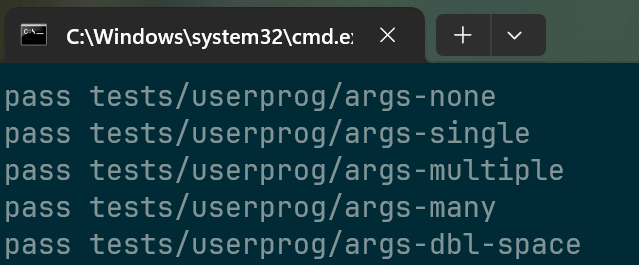
\includegraphics[width=0.38\textwidth]{img6/pass.png}
    \caption{参数传递}
    \label{fig:lab6-1}
\end{figure}

但实际上我基本上算只能完成了参数传递,因为我需要阶段性成果所以借鉴了博主的文章,残留的 \texttt{process\_wait} 仍未实现,而是通过写了 \textbf{while(1)} 的死循环来让线程不退出,最后才通过的检查点。

现在,让我们清除这部分内容,完成完整的系统调用!

\subsection{Mission 2: Process Termination Messages}

\subsubsection{定义 thread.h 结构体}

最初,我们只完成了参数传递,而忽略了实验手册中的另一个 Mission,这里它要求我们实现进程终止消息。
想要把所有的 Checkpoints 给过了,想必这一部分肯定是必不可少的,故现在把这个跳过的部分给补全。

在用户进程终止时打印一条信息,这个操作于 \texttt{process\_exit()} 中进行最好。
进程名称在线程创建时有被记录到 \texttt{name} 成员中,但是退出状态目前是没有记录的。
于是 \texttt{exit\_status} 成员的作用应运而生,然而它的更新与系统调用(\texttt{exit} 等)有关,而上一次实验报告仅注重于参数传递的部分。

实验手册中也指出了这一点,这是我当时跳过的主要原因:

\begin{figure}[H]
    \centering
    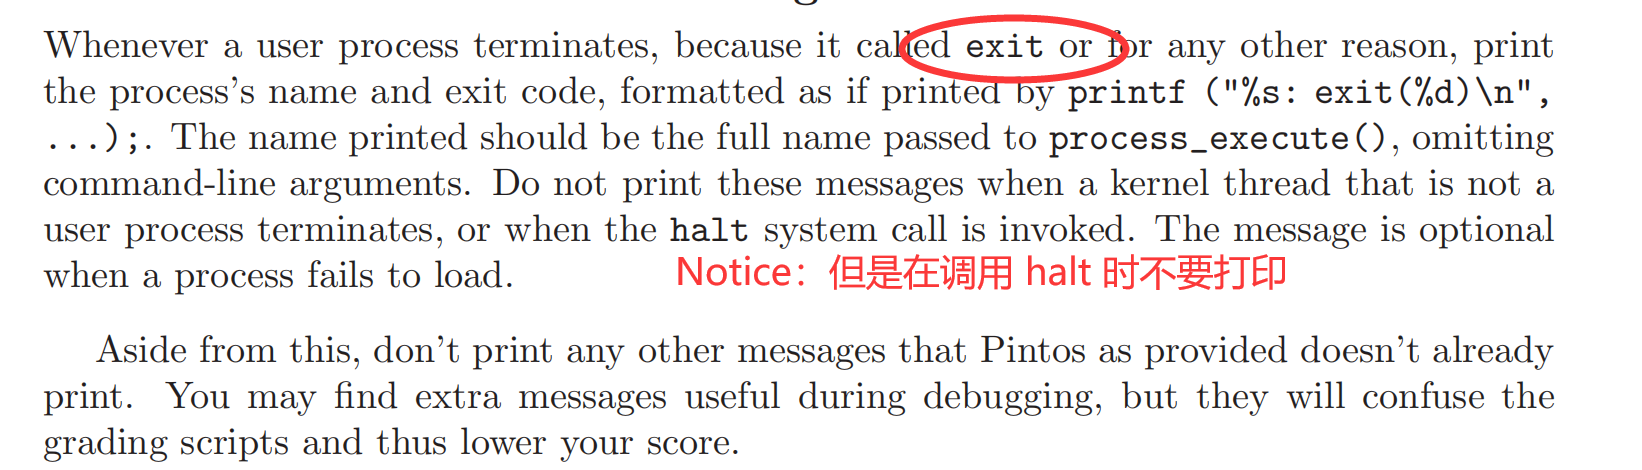
\includegraphics[width=0.68\textwidth]{img6/todo.png}
    \caption{Mission 2: Process Termination Messages}
    \label{fig:lab6-2}
\end{figure}

既然要打印返回值,那我们可以在初始化线程时,
将 \texttt{exit\_status} 作为参数传递给 \texttt{process\_exit()},这样就可以在 \texttt{process\_exit()} 中打印返回值了。

线程在退出时,我们查阅这部分相关的代码进行分析,注释中高亮了我提到的部分:

\begin{lstlisting}[language=C, title = thread\_exit()]
    /** Deschedules the current thread and destroys it. Never returns to the caller. */
    void thread_exit (void) {
        ASSERT (!intr_context ());
    #ifdef USERPROG
        process_exit();
        // 在用户进程退出时,process_exit() 负责关闭文件、释放页表等资源
        // 如果是内核线程,则无需调用 process_exit()
    #endif
    /* Remove thread from all threads list, set our status to dying,
      and schedule another process.  That process will destroy us
      when it calls thread_schedule_tail(). */
        intr_disable();
        list_remove(&thread_current()->allelem);
        thread_current()->status = THREAD_DYING;
        schedule();
        NOT_REACHED();
    }
\end{lstlisting}

\begin{cth}
    查阅文档可得:\href{https://uchicago-cs.github.io/mpcs52030/switch.html}{\underline{https://uchicago-cs.github.io/mpcs52030/switch.html}},
    
    用户进程只有一个线程,而内核进程是 Multithreading 的,在下图的 Switching Between processes 中有提到一些这部分的内容。
    若是用户进程,则会调用 \texttt{process\_exit()} 终止整个进程,
\end{cth}

\begin{figure}[H]
    \centering
    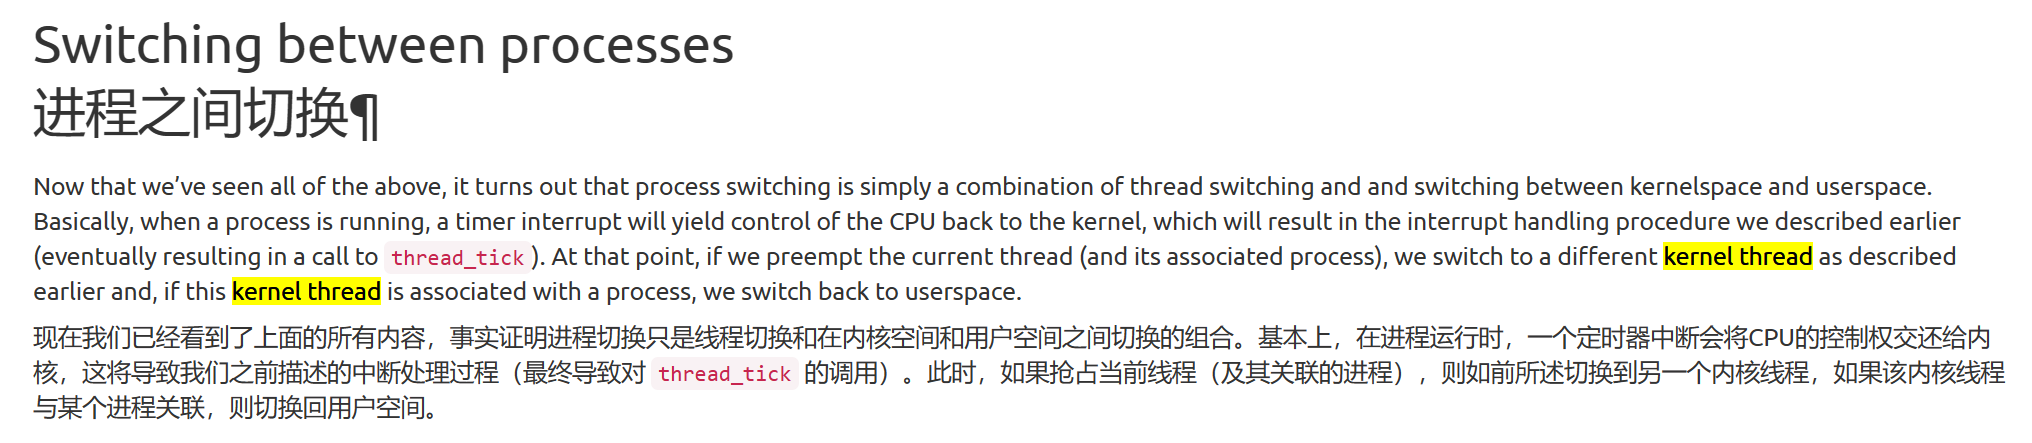
\includegraphics[width=0.8\textwidth]{img6/info1.png}
    \caption{Switching Between processes}
    \label{fig:lab6-3}    
\end{figure}

首先,我们在 \texttt{thread structure} 中定义一个 \texttt{exit\_status} 成员。

这里为了后面的方便,我直接把 PPT 中要求我们添加的数据结构放进来了:

按照 PPT 要求,在 \texttt{thread.h} 中新增结构体变量:

\begin{figure}[H]
    \centering
    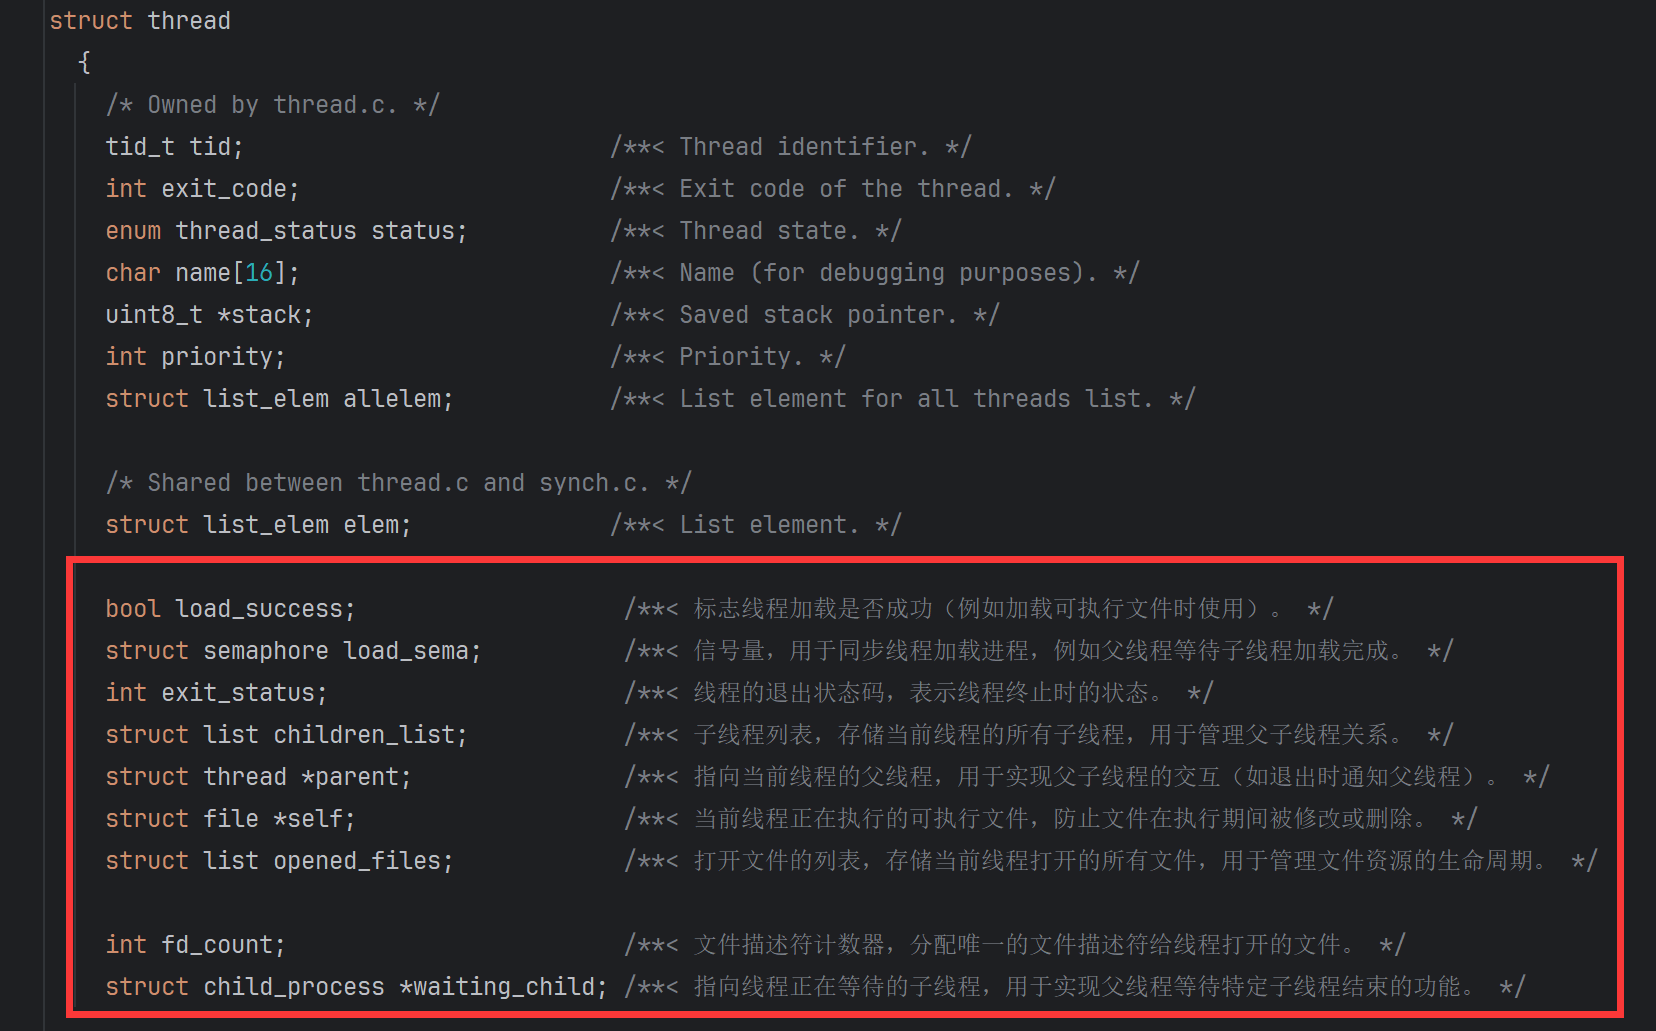
\includegraphics[width=0.8\textwidth]{img5/new.png}
    \caption{thread.h}
    \label{fig:thread}
\end{figure}

同时定义全局锁:\textbf{struct lock filesys\_lock},用于文件系统操作的同步。该结构体 \texttt{lock} 位于 \textbf{synch.h} 中。

当然,不能忘记了子进程的结构体定义:

\begin{lstlisting}[language=C,title= child\_process]
struct child_process {
    int tid;                     /**< 子进程的线程 ID。 */
    bool if_waited;              /**< 子进程是否已被父进程等待。 */
    int exit_status;             /**< 子进程的退出状态。 */
    struct list_elem child_elem; /**< 子进程的元素。 */
    struct semaphore wait_sema;  /**< 等待子进程退出的信号量。 */
};
\end{lstlisting}

对于上一次编写的系统调用,因为有文件相关的功能加入,所以一部分代码是不通的,要注意不能完全沿用上一次报告中的部分系统调用的代码。

定义之后,我们可以先在 \texttt{init\_thread()} 中将其初始化,将其添加到 \texttt{thread} 的结构体中,以供后续调用和修改。

\begin{lstlisting}[language=C,title= init\_thread]
    static void init_thread (struct thread *t, const char *name, int priority) {
        ...

        list_init(&t->children_list); // child_process 结构体的列表
        t->parent = running_thread(); // 正在运行的线程设置为新线程的父线程
        list_init(&t->opened_files); // 初始化线程的 opened_files 链表,记录线程打开的所有文件
        t->fd_count=2; // 标准输入、输出、错误文件描述符
        t->exit_status = INIT_EXIT_STAT; // 退出状态设初值
        sema_init(&t->load_sema,0); // 初始化线程的 load_sema 信号量 = 0
        t->waiting_child=NULL; // 没在等待子线程
        t->self=NULL;
        list_insert_ordered(&all_list, &t->allelem, (list_less_func *)&compare_priority, NULL);
        // 插入至维护的全局线程列表中
    }
\end{lstlisting}

为什么在这里设置 \texttt{fd\_count = 2} 呢?主要在文档中有提到(在 \texttt{open} 相关的系统调用部分):

\begin{figure}[H]
    \centering
    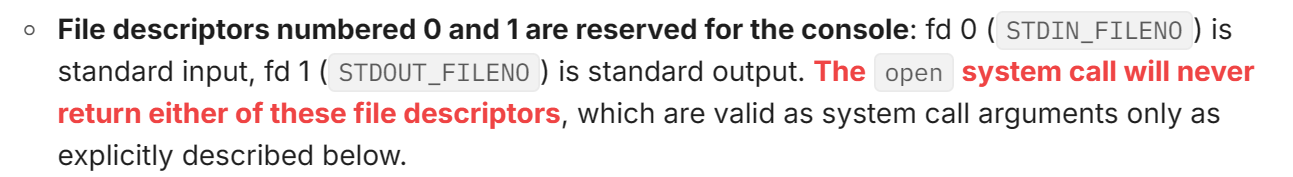
\includegraphics[width=0.8\textwidth]{img6/not01.png}
    \caption{FD != 0 or 1}
    \label{fig:lab6-4}
\end{figure}

\begin{thm}{Count = 2}{Count = 2}
    文件描述符(File Descriptor,简称 fd)是操作系统中分配给线程(或进程)打开文件的唯一标识。
    
    在 Pintos 中,文件描述符 0 和 1 通常被保留:

    \begin{itemize}
        \item fd = 0:标准输入:stdin
        \item fd = 1:标准输出:stdout
    \end{itemize}
    因此,新打开的文件描述符从 2 开始分配,确保每个文件有唯一的标识符。
\end{thm}

\vspace{0.3cm}

\begin{cth}
另外,Pintos 中维护了一个全局线程列表,记录所有线程(用户进程和内核线程),所以我们可以使用 \texttt{list\_insert\_ordered()} 函数将新创建的线程插入到正确的位置。
\end{cth}

\subsubsection{完善 Mission 2 代码}

添加了 \texttt{exit\_status} 成员后,我们要初始化它,在进程初始化(\texttt{init\_thread()})时,给它赋予一个初始值。

\begin{cth}
在操作系统中,父进程需要跟踪和管理子进程的状态信息,例如:

子进程的退出状态,
是否已经被父进程等待过(\texttt{if\_waited}),以及父子进程间需要的同步机制。

\vspace{0.5cm}

在 Pintos 中,父进程通过 \texttt{struct child\_process} 来记录每个子进程的相关信息,这样父进程可以:
在子进程退出时查询其退出状态。
调用 \texttt{wait()} 系统调用等待子进程完成。
避免子进程的状态信息丢失(因为子进程可能比父进程先退出)。

\end{cth}

\begin{lstlisting}[language=C,title= init\_thread]
    #define INIT_EXIT_STATUS -1 // 注意:这里要赋予一个初始值,否则会导致进程退出时打印出未初始化的地址
    tid_t thread_create (const char *name, int priority, thread_func *function, void *aux) {
        tid_t tid;
        
        /* Allocate thread. */
        t = palloc_get_page (PAL_ZERO);
        if (t == NULL)
        return TID_ERROR;

        /* Initialize thread. */
        init_thread (t, name, priority);
        tid = t->tid = allocate_tid ();

        struct child_process* c = malloc(sizeof(*c)); 
        c->tid = tid;
        c->exit_status = t->exit_status;
        // 将当前线程(t,即子进程)的退出状态保存在子进程的结构体中,供父进程稍后访问。
        // 本设计是为了支持 wait() 系统调用的实现。
        c->if_waited = false;
    }
\end{lstlisting}

万事俱备,此时只需要在 \texttt{process\_exit()} 函数中加入终止消息的打印句子即可:

\begin{lstlisting}[language=C,title= process\_exit()]
    // Free the current process's resources.
    void process_exit (void) {
        struct thread *current_thread = thread_current();
        uint32_t *pd;

        int exit_status = current_thread->exit_status;
        if (exit_status == INIT_EXIT_STAT) exit_process(-1);
        // exit_status == INIT_EXIT_STAT,说明当前进程还没有设置退出状态
        // 可能是由于异常退出或未正确调用 exit()。

        printf("%s: exit(%d)\n",current_thread->name,exit_status);
    }
\end{lstlisting}

\begin{cth}
    其实,如果其他实现全部正确,只需要最后一行的 \texttt{printf()}已经足够了,前面的 \texttt{if} 语句中,如果没有加载成功一个进程,即状态仍然为自定义的状态,
    调用 \texttt{exit\_process(-1)} 将进程的退出状态强制设置为 $-1$,表示错误退出(例如因非法操作或其他未定义行为导致的退出)。
    这里加上了是为了解决一些可能出现的问题,让报错更加合理。
\end{cth}

在实现了之后的系统调用后,我回来这里补充了一张图片,以证明 Mission 2 已经完成:

按照 PPT 中的测试方法,随意选择一个进程,看看是否会输出进程中止信息:

\begin{figure}[H]
    \centering
    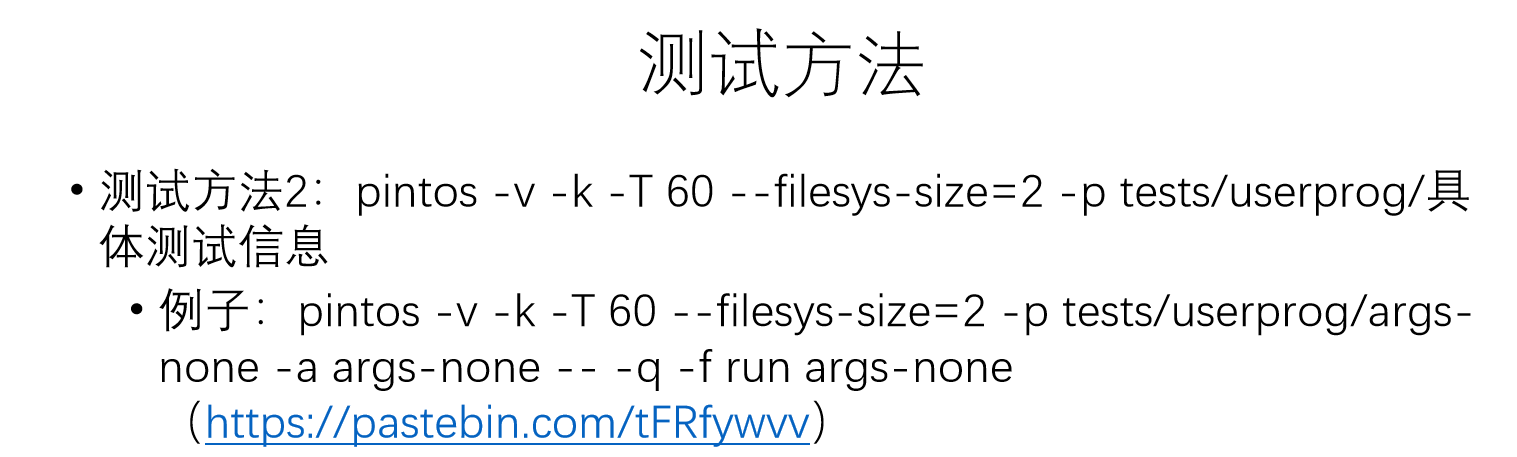
\includegraphics[width=0.52\textwidth]{img6/tip1.png}
    \caption{PPT 中的示例测试命令}
    \label{fig:lab6-5}
\end{figure}

使用以上命令后,得到了如下的结果,愉悦地发现已经实现了参数传递和进程终止信息了!

\begin{figure}[H]
    \centering
    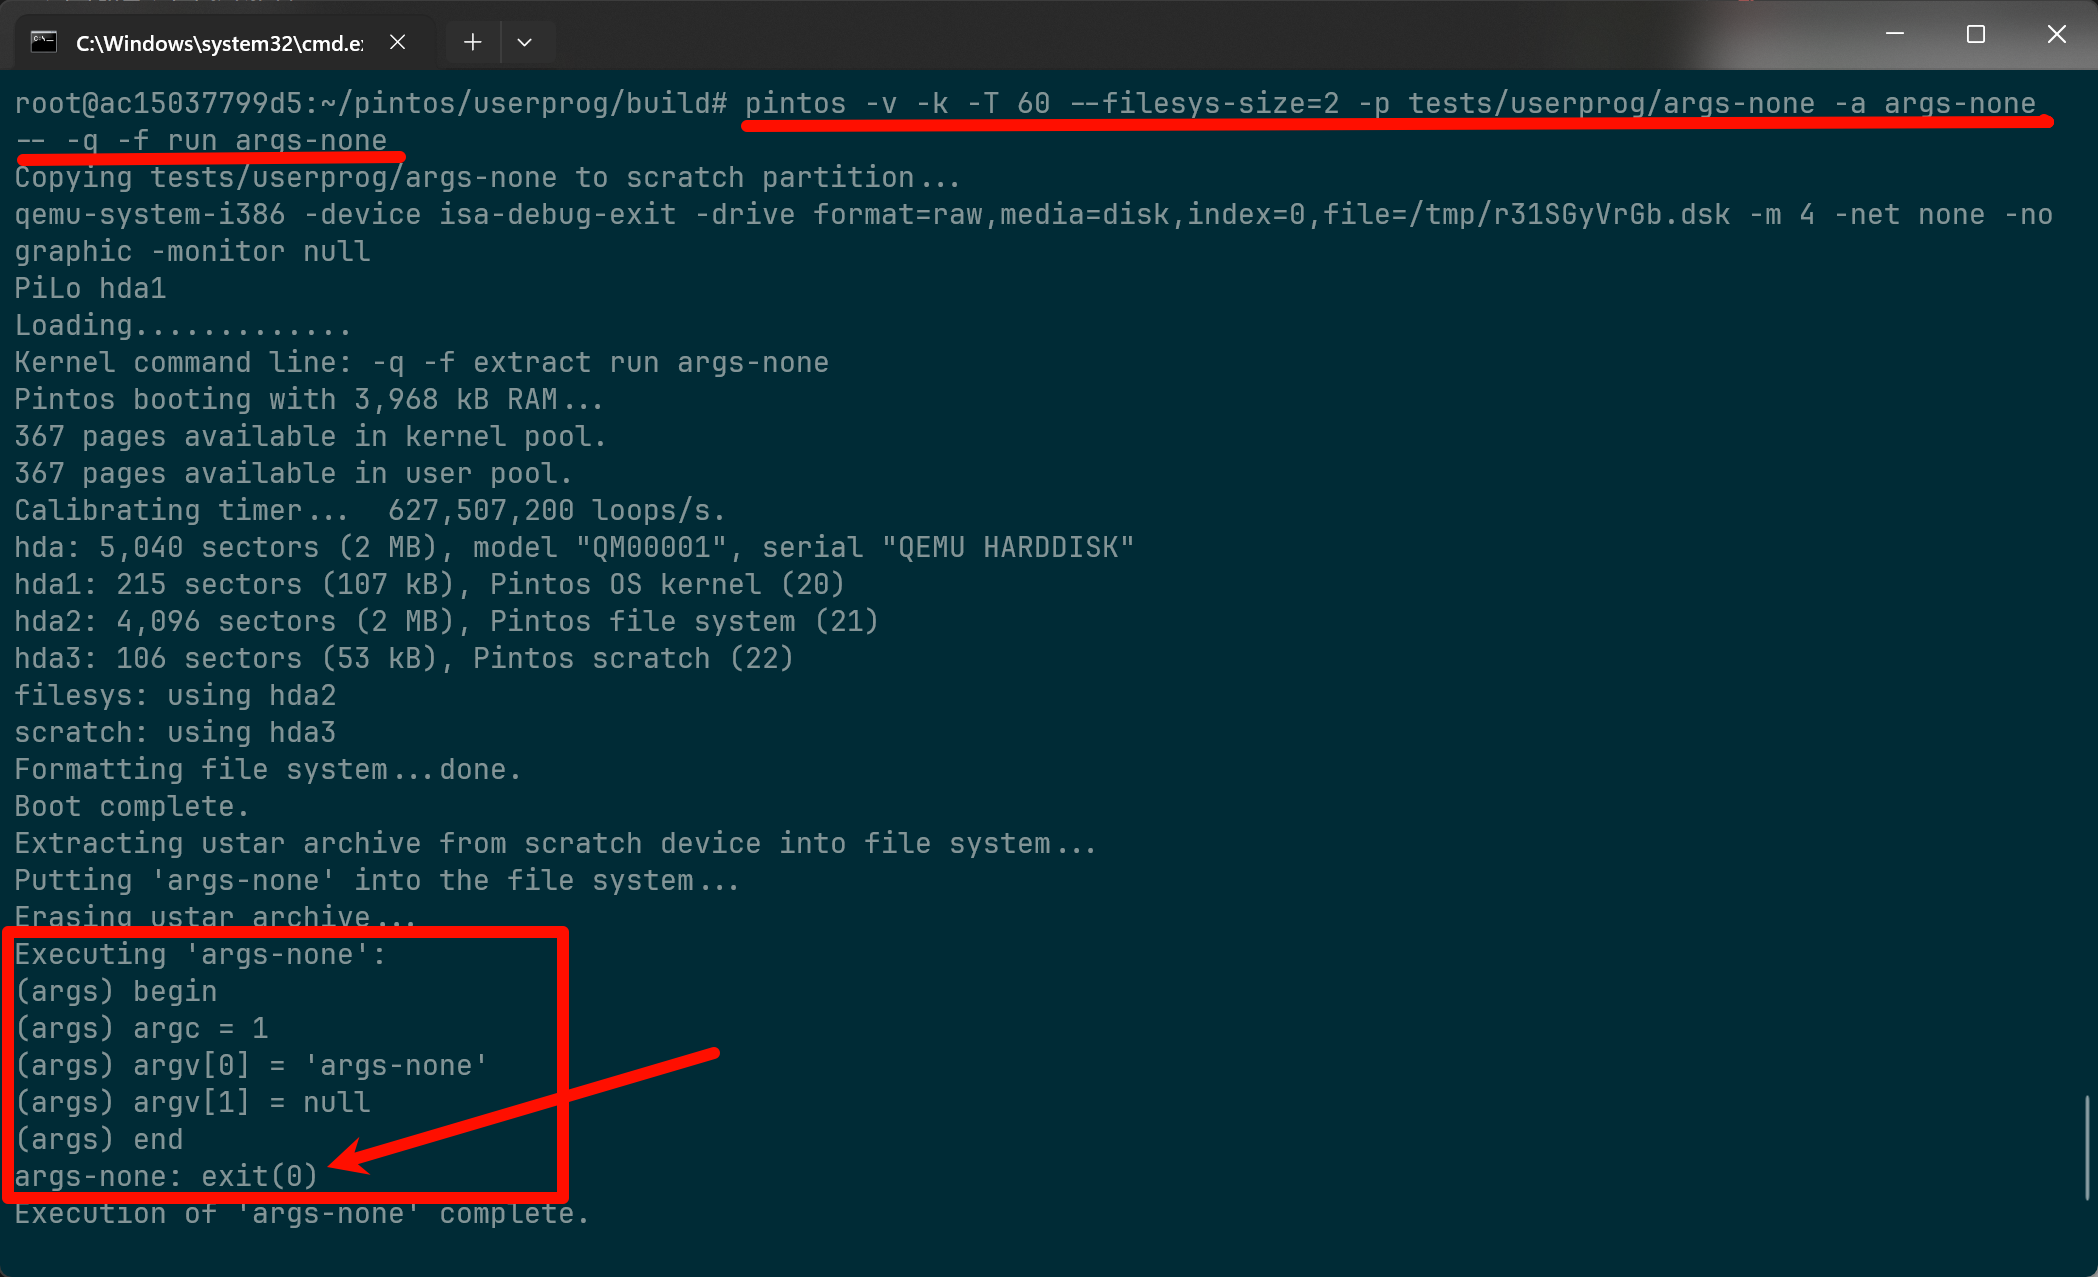
\includegraphics[width=0.6\textwidth]{img6/done.png}
    \caption{Mission 2 完成}
    \label{fig:lab6-4}
\end{figure}

结果完好!代表这一部分已完成!

\subsection{Mission 4: System Calls}

官方手册中的 Mission 3 是参数传递,在之前已经做了,Mission 2 是之前留着尚未实现的,现在补充完成了,接下来我们着手开始最难的部分:系统调用。

手册中对于每一个需要实现的系统调用都写了详细的注释,就不全部搬过来了,按照 Lab 5 - Userprog Part 1 中写过的代码做一些分析和修改。

\subsubsection{Syscall Handler}

为了让逻辑更具合理性,还是搬一部分上一节的内容来:

除了我们要实现的 \texttt{userprog/syscall.c},在 \texttt{lib/user} 文件夹下,还有一对 \texttt{syscall.h} 和 \texttt{syscall.c} 文件

\begin{ctt}
这组文件,是 提供给用户的系统调用接口,其通过 int \$0x30 
中断指令以唤起一个系统调用,
最终会落入 userprog/syscall.c 的 syscall\_handler() 函数中。
\end{ctt}

注意到,其 enum 中定义了不同的系统调用的序号(这里只截取与 Project 2 相关的):

\begin{lstlisting}[language=C, title= syscall.h]
    enum {
        /* Projects 2 and later. */
        SYS_HALT,                   /**< Halt the operating system. */
        SYS_EXIT,                   /**< Terminate this process. */
        SYS_EXEC,                   /**< Start another process. */
        SYS_WAIT,                   /**< Wait for a child process to die. */
        SYS_CREATE,                 /**< Create a file. */
        SYS_REMOVE,                 /**< Delete a file. */
        SYS_OPEN,                   /**< Open a file. */
        SYS_FILESIZE,               /**< Obtain a file's size. */
        SYS_READ,                   /**< Read from a file. */
        SYS_WRITE,                  /**< Write to a file. */
        SYS_SEEK,                   /**< Change position in a file. */
        SYS_TELL,                   /**< Report current position in a file. */
        SYS_CLOSE,                  /**< Close a file. */
    };
\end{lstlisting}

故我们需要在 \textbf{syscall\_handler()} 中实现分发:
根据类型分发给各个具体处理函数,逐个实现。
返回值要放在 EAX 中传回调用者。

在官方文档中也有这一部分的内容:

\begin{figure}[H]
    \centering
    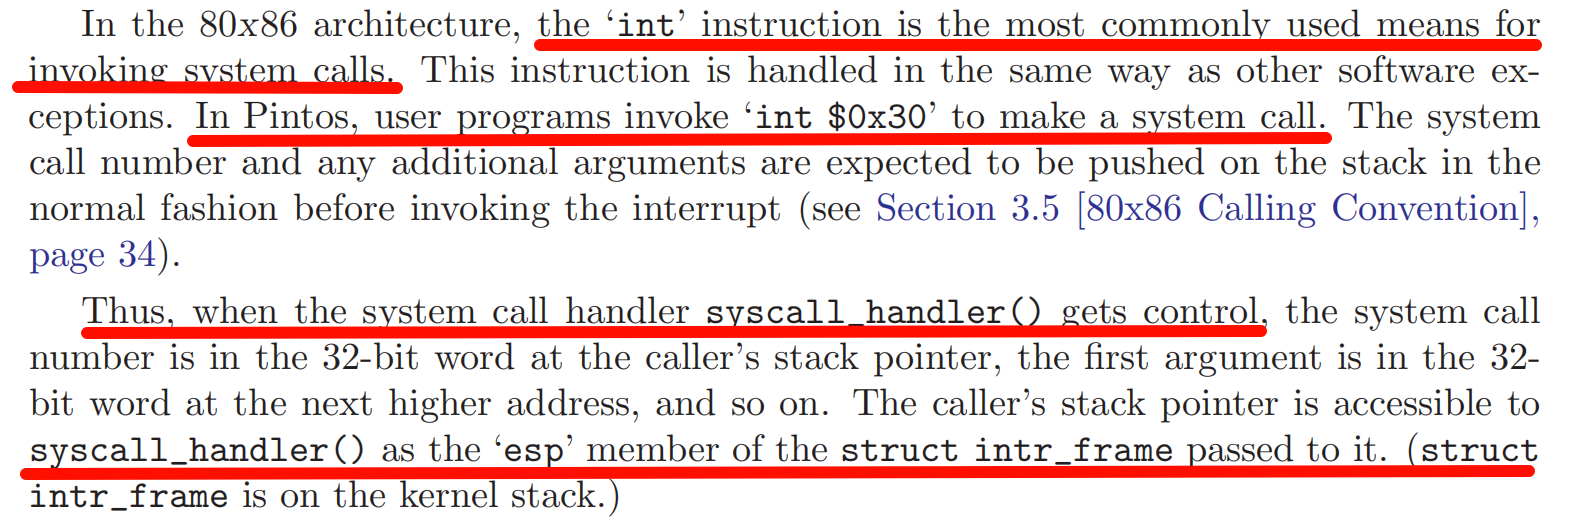
\includegraphics[width=0.68\textwidth]{img6/handler.png}
    \caption{Handler}
    \label{fig:lab6-6}
\end{figure}


\begin{ctt}
    在 Pintos 中,\texttt{struct intr\_frame} 是用来保存中断处理器状态的结构体。在系统调用返回时,通常会将结果值存储到 f->eax 中,因为这是 x86 架构的约定——返回值通过 eax 寄存器传递。
    
    \vspace{0.5cm}

    对于系统调用 \texttt{SYS\_EXIT},需要返回一个退出码到用户进程,返回值就需要存放到 f->eax 中。
    类似地,\texttt{SYS\_WRITE} 也会将写入的字节数返回到 f->eax。
\end{ctt}

\begin{lstlisting}[language=C, title= syscall.c]
    static void syscall_handler (struct intr_frame *f UNUSED) {
        int *p = f->esp;
        is_valid_addr(p);
        int system_call = *p;
        switch (system_call) {
            case SYS_HALT: syscall_halt(); break;
            case SYS_EXIT: syscall_exit(f); break; // 直接关机,不需要返回值,故是 void function
            case SYS_EXEC: f->eax = syscall_exec(f); break;
            case SYS_WAIT: f->eax = syscall_wait(f); break;
            case SYS_CREATE: f->eax = syscall_creat(f); break;
            case SYS_REMOVE: f->eax = syscall_remove(f); break;
            case SYS_OPEN: f->eax = syscall_open(f); break;
            case SYS_FILESIZE: f->eax = syscall_filesize(f); break;
            case SYS_READ: f->eax = syscall_read(f); break;
            case SYS_WRITE: f->eax = syscall_write(f); break;
            case SYS_SEEK: syscall_seek(f); break; // 调整文件指针的位置,也不需要返回值
            case SYS_TELL: f->eax = syscall_tell(f); break;
            case SYS_CLOSE: syscall_close(f); break;
            default: printf("Default %d\n",*p);
        }
    }
\end{lstlisting}

在上方的函数中,有一些函数是不需要返回值的,这些 \texttt{void function} 在定义的时候要注意一下。

我们把这些函数定义好,放在 \texttt{syscall.c} 的顶部,先声明这个函数的存在,然后搭建好函数框架,对没有实现的函数我们可以使用 \texttt{return -1;} 语句来解决(类似 Python 中的 Pass 的效果)。

\begin{lstlisting}[language=C]
    void exit_process(int status);
    void *is_valid_addr(const void *vaddr);
    void syscall_exit(struct intr_frame *f);
    int syscall_exec(struct intr_frame *f);
    int syscall_wait(struct intr_frame *f);
    int syscall_creat(struct intr_frame *f);
    int syscall_remove(struct intr_frame *f);
    int syscall_open(struct intr_frame *f);
    int syscall_filesize(struct intr_frame *f);
    int syscall_read(struct intr_frame *f);
    int syscall_write(struct intr_frame *f);
    void syscall_seek(struct intr_frame *f);
    int syscall_tell(struct intr_frame *f);
    void syscall_close(struct intr_frame *f);
    void syscall_halt(void);
    
    // 搭建函数框架,什么也不做,保证编译成功
    // For Example:
        static void syscall_remove(struct intr_frame *f) {
            return -1;  // 直接返回错误,什么都不做
        }
\end{lstlisting}

其次,Pintos 中已经使用了 \texttt{syscall\_init} 将中断处理函数注册到寄存器:

\begin{lstlisting}[language=C, title= init.c]
    void syscall_init (void) {
        intr_register_int (0x30, 3, INTR_ON, syscall_handler, "syscall");
    }
\end{lstlisting}

另外要注意的是,Pintos 中不允许在系统调用中使用 malloc() 函数:

\begin{figure}[H]
    \centering
    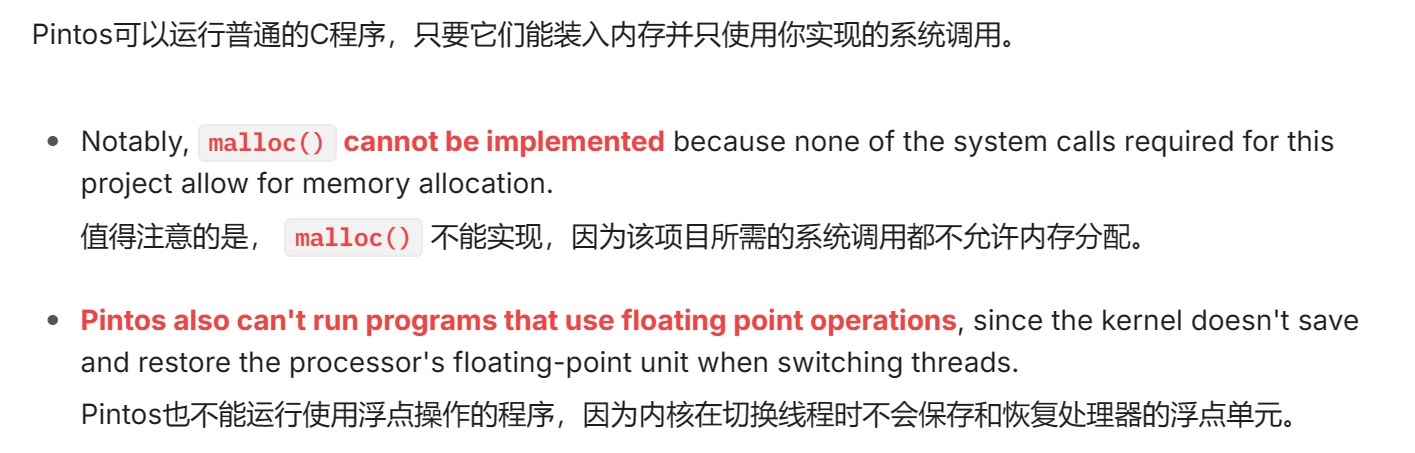
\includegraphics[width=0.5\textwidth]{img5/warning.png}
    \caption{malloc()}
    \label{fig:malloc}
\end{figure}

\subsubsection{处理内存非法访问}

PPT 中的提示了使用 \texttt{syscall\_create} 来实现,这一部分有检查内存非法访问的功能,我们先把这些代码搬过来为己所用。

\begin{figure}[H]
    \centering
    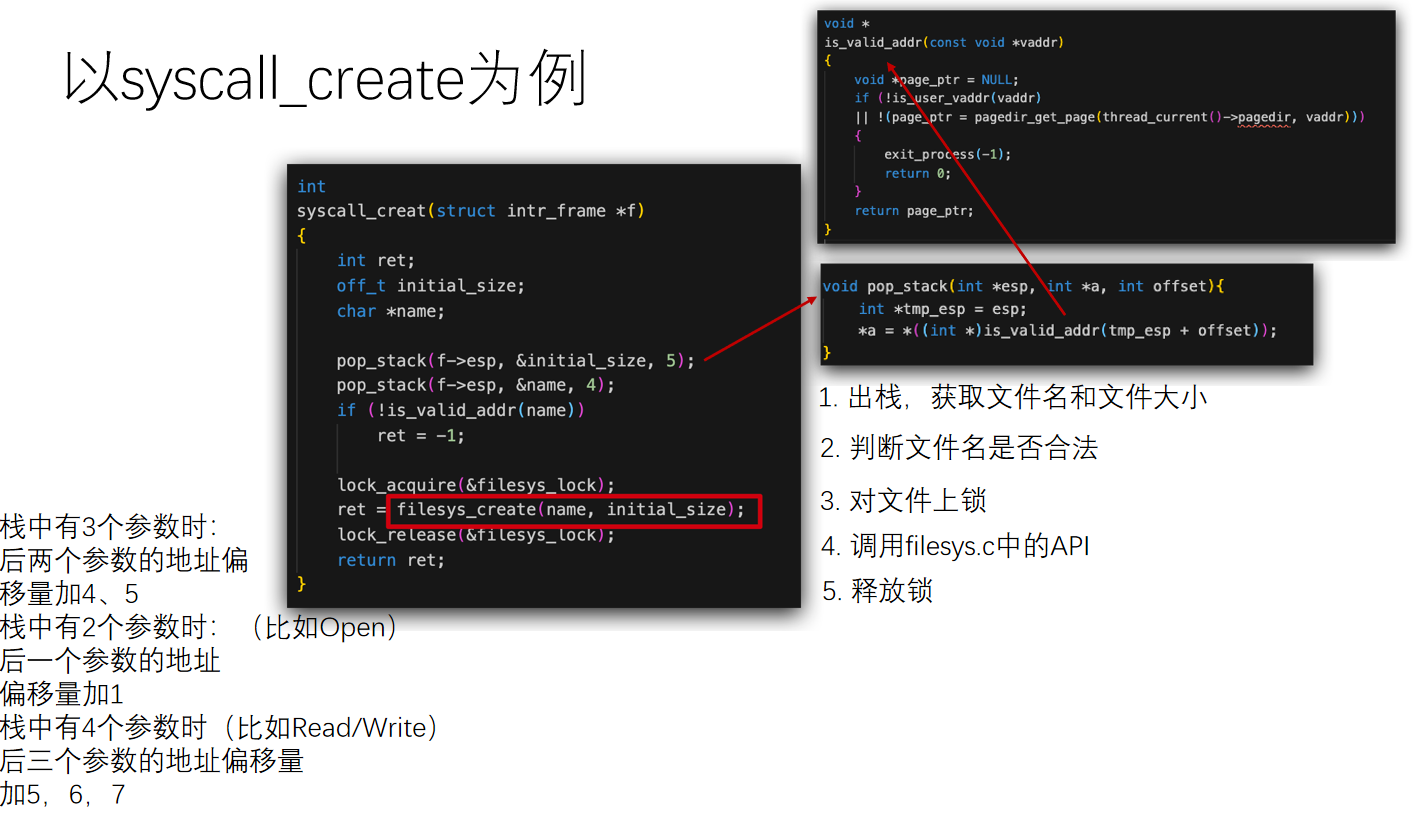
\includegraphics[width=0.8\textwidth]{img5/ppt.png}
    \caption{PPT}
    \label{fig:check}
\end{figure}

为了保证内核不受到破坏,需要立即终止发出非法指针请求的进程。查
看 \texttt{userprog/pagedir.c} 和 \texttt{threads/vaddr.h},可以发现已经为我们定义了以下两个函数:

\begin{lstlisting}[language=C,title= pagedir\_get\_page()]
    /* Looks up the physical address that corresponds to user virtual address UADDR in PD.
    Returns the kernel virtual address
    corresponding to that physical address, or a null pointer if UADDR is unmapped. */
    void *pagedir_get_page (uint32_t *pd, const void *uaddr) {
        uint32_t *pte;
        ASSERT (is_user_vaddr (uaddr));
        pte = lookup_page (pd, uaddr, false);
        if (pte != NULL && (*pte & PTE_P) != 0)
            return pte_get_page (*pte) + pg_ofs (uaddr);
        else
            return NULL;
   }
\end{lstlisting}

\begin{lstlisting}[language=C,title= is\_user\_vaddr()]
    /* Returns true if VADDR is a user virtual address. */
    static inline bool is_user_vaddr (const void *vaddr) {
        return vaddr < PHYS_BASE;
    }
\end{lstlisting}

除了空指针以外,这就是最常见的两个异常情况。当出现异常的时候都会返回异常信息。
可以借助这两个函数来实现内存访问的安全控制。

我们可以跟着这个思路来编写代码:

\begin{cth}
检查传入的虚拟地址是否是用户空间的有效地址:

使用 \texttt{is\_user\_vaddr} 判断地址是否在用户地址范围内。如果是有效的用户地址,则使用 \texttt{pagedir\_get\_page} 从当前线程的页目录中获取该虚拟地址对应的物理页指针。

如果地址无效或无法找到对应的物理页,则调用 \texttt{exit\_process(-1)} 退出当前进程。
\end{cth}

\begin{lstlisting}[language=C, title= syscall\_create()]
    void *is_valid_addr(const void *vaddr) {
        void *page_ptr = NULL;
        if (!is_user_vaddr(vaddr) || !(page_ptr = pagedir_get_page(thread_current()->pagedir, vaddr))) {
            exit_process(-1); // 地址无效,退出进程
            return 0;
        }
    return page_ptr;     // 地址有效,返回物理页指针
    }
\end{lstlisting}

如果地址无效则以异常状态中止进程,有效则返回物理地址。

再编写 pop\_stack() 函数,用于从栈中取得元素,方便取得参数:

\begin{lstlisting}[language=C, title= pop\_stack()]
    void pop_stack(int *esp, int *a, int offset){
        int *tmp_esp = esp;
        *a = *((int *)is_valid_addr(tmp_esp + offset));
    }
\end{lstlisting}

这里是因为 Pintos 使用的是 4 字节对齐,所以 offset 参数可以方便地使用整数来取得参数。

\begin{figure}[H]
    \centering
    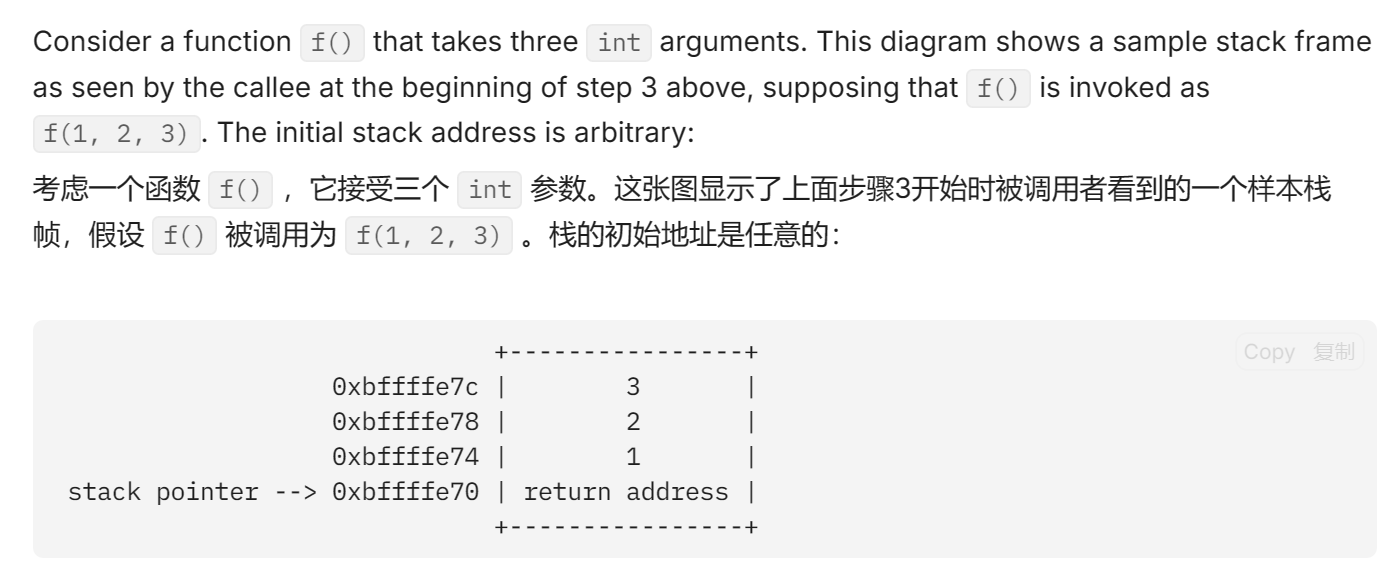
\includegraphics[width=0.65\textwidth]{img5/stackpointer.png}
    \caption{栈指针}
    \label{fig:stack}
\end{figure}

\subsubsection{Halt}

本系统调用是最简单的,这里只需要简单地调用 \textbf{devices/shutdown.c} 下的函数接口即可:

用于通过调用底层硬件接口直接关闭计算机(在模拟环境中是关闭虚拟机或退出 \texttt{QEMU} 模拟器)。

\begin{lstlisting}[language=C]
    void syscall_halt(void){
        shutdown_power_off();
    }
\end{lstlisting}

\subsubsection{Exit}

本系统调用的主要目的是终止当前用户程序,返回到内核:

可以在 Pintos 的 Gitbook 上查阅到更多信息:\href{https://pkuflyingpig.gitbook.io/pintos/project-description/lab2-user-programs/your-tasks}{\underline{Lab2-User-Program/your-tasks}}

\begin{figure}[H]
    \centering
    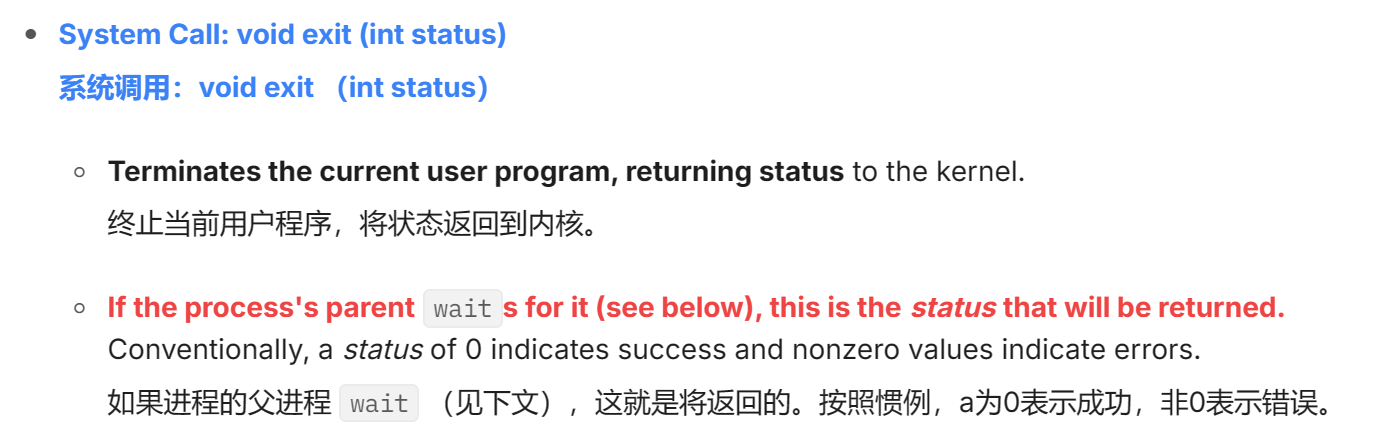
\includegraphics[width=0.65\textwidth]{img6/exit.png}
    \caption{Exit Doc}
    \label{fig:exit}
\end{figure}

当我们不管父进程和子进程之间的关系时,上一份实验报告中的简单实现如下所示:

\begin{lstlisting} [language=C]
    static void syscall_exit(struct intr_frame *f) {
        // exit_code在系统调用之后被解析为参数
        int exit_code = *(int *)(f->esp + sizeof(void *));
        thread_current()->exit_status = exit_code;
        thread_exit();
    }
\end{lstlisting}

这样的设计是基于 Pintos 中,当用户程序调用系统调用(例如 \texttt{exit()})时,用户程序的参数会按照约定存储在栈中。
\texttt{f->esp} 指向栈顶,此时栈的布局大致如下:

\begin{lstlisting}
             +--------------------+
             | system call number |  <--- f->esp (指向系统调用号)
             +--------------------+
             |    exit_code       |  <--- f->esp + 4 (紧随其后的第一个参数)
             +--------------------+    
\end{lstlisting}

但一旦需要考虑父子进程,那么问题就变得复杂起来了。
我们先根据之前的 \texttt{pop\_stack()} 函数从栈顶获取 \texttt{status},遍历子进程,
使进程调用 \texttt{thread\_exit()} 退出。

将函数改写成这样(调用跟着 PPT 的提示实现的 \texttt{pop\_stack()} 函数)

\begin{lstlisting}[language=C, title= syscall\_exit()]
    static void syscall_exit(struct intr_frame *f) {
        int status;
        pop_stack(f->esp, &status, 1); // 和上面的实现一样,从栈顶获取状态码
        exit_process(status);
    }
\end{lstlisting}

其中,我们可以把子函数 \texttt{exit\_process()} 函数定义成:

\begin{lstlisting}[language=C, title= exit\_process()]
    void exit_process(int status) {
        /*
        * 1. 将当前线程的退出状态更新到父进程的子进程列表中。
        * 2. 标记当前线程的子进程状态为已等待(if_waited = true)。
        * 3. 调用 thread_exit() 彻底终止当前线程。
        */

        struct child_process *cp; // 指向当前进程在父进程 chilren_list 中对应子进程的状态
        struct thread *cur_thread = thread_current(); // 当前的线程就是即将调用 Exit() 系统调用的进程
    
        enum intr_level old_level = intr_disable(); // 关闭中断,这里是照猫画虎
        // 存储了所有子进程的 struct child_process 结构体
        for (struct list_elem *e = list_begin(&cur_thread->parent->children_list);
            e != list_end(&cur_thread->parent->children_list);
            e = list_next(e)) {
            cp = list_entry(e, struct child_process, child_elem); // 从链表元素 e 获取结构体
            if (cp->tid == cur_thread->tid) { // 若线程与子进程的 TID 相匹配
                cp->if_waited = true; // 那么当前线程对应的子线程已被等待过了,可以防止父进程重复调用 wait()
                cp->exit_status = status; // 将退出状态保存到子进程的状态中,父进程就可以通过 exit() 获取
            }
        }

        cur_thread->exit_status = status; // 记录退出状态,方便父线程查询
        intr_set_level(old_level); // 恢复之前的中断状态,确保系统中断处理继续正常运行
        thread_exit(); // 大功告成,退出当前线程!
    }
\end{lstlisting}

如此,便完整实现了 \texttt{syscall\_exit()} 的系统调用。

\subsubsection{Exec}

从 PPT 中我们可以获得一些 References:

\begin{figure}[H]
    \centering
    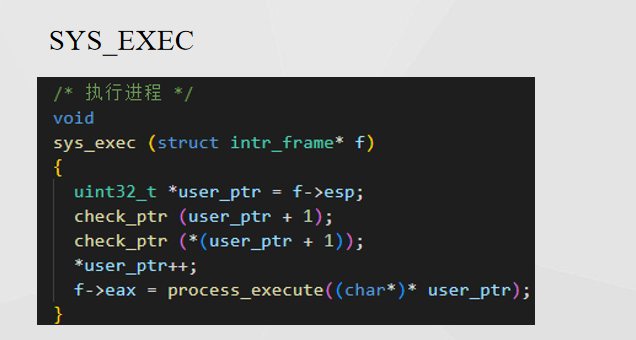
\includegraphics[width=0.4\textwidth]{img6/ref-exec.png}
    \caption{Exec-Ref}
    \label{fig:exec}
\end{figure}

\begin{cth}

这里的检查指针的操作其实我们直接用之前写的函数 \texttt{is\_valid\_addr()} 来检查即可,同样地,也是从栈顶拿取元素。

当 \texttt{syscall\_exec(file\_name)}被调用的时候。首先应当确认传递来的参
数 \texttt{file\_name} 是否为有效的。如果有效,则执行 \texttt{exec\_process()}

\end{cth}

\begin{lstlisting}[language=C, title= syscall\_exec()]
    int syscall_exec(struct intr_frame *f) {
        char *file_name = NULL;
        pop_stack(f->esp, &file_name, 1);
        if (!is_valid_addr(file_name))
            return -1;
        return exec_process(file_name);
    }
\end{lstlisting}

到此还不够,这只是搭好了一个框架而已,不妨让我们打开 Pintos Guidebook 看看要求:

\begin{figure}[H]
    \centering
    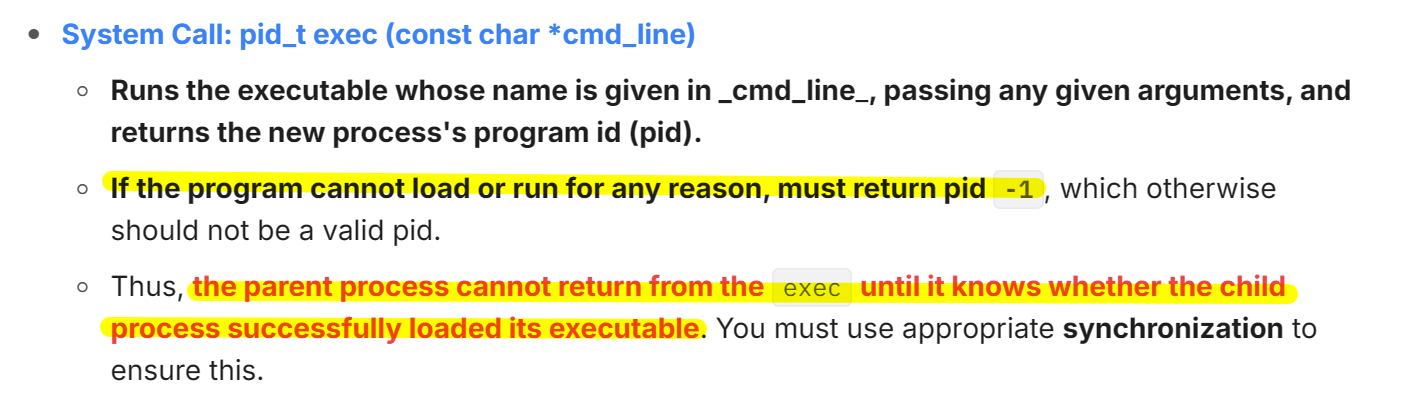
\includegraphics[width=0.65\textwidth]{img6/exec_request.png}
    \caption{Request-Exec}
\end{figure}

根据这里提供的信息:

\begin{mdframed}[backgroundcolor=gray!10, linewidth=0.5pt, roundcorner=5pt]
    
    \textit{1. 如果程序由于任何原因不能加载或运行,必须返回 $pid = -1$};

    \textit{2. 父进程在知道子进程是否成功加载其可执行文件之前,不能从 \texttt{exec} 返回}。
\end{mdframed}

\begin{cth}
    \texttt{exec\_process} 函数的核心逻辑是检查一个用户进程的可执行文件是否存在,并确保文件系统的线程安全。

    \vspace{0.2cm}

    整个执行过程都是通过 \texttt{filesys\_lock} 来实现互斥访问,为了保证不并行执行多个文件访问,
    通过获取文件系统锁,防止多个线程同时访问文件系统导致竞争条件。

    \vspace{0.2cm}

    如果文件不存在,则立即释放锁并返回 $-1$,表明进程无法启动;如果文件存在,则关闭文件释放锁,随后执行传入的文件。
\end{cth}

按照这个设计思路,子函数 \texttt{exec\_process()} 如下,这是解决该调用最核心的函数:

\begin{lstlisting}[language=C, title= exec\_process()]
    int exec_process(char *file_name) {
        /**
        * 尝试执行一个用户进程对应的可执行文件。如果文件存在,则通过 process_execute() 创建并执行进程;
        * 否则返回 -1,表示文件不存在。
        *
        * Parameters:file_name: 包含可执行文件名和参数的字符串。
        * Return:成功时返回新进程的线程 ID (tid),失败时返回 -1。
        */
        int tid;

        // 获取文件系统锁,确保文件系统操作的线程安全
        lock_acquire(&filesys_lock);
    
        // 为 file_name 分配临时存储,确保不修改原始参数
        char *name_tmp = malloc(strlen(file_name) + 1);
        strlcpy(name_tmp, file_name, strlen(file_name) + 1);
    
        char *tmp_ptr;
        name_tmp = strtok_r(name_tmp, " ", &tmp_ptr);  // 使用 strtok_r 提取文件名(忽略参数部分)
        struct file *f = filesys_open(name_tmp);      // 打开文件以检查文件是否存在
        
        if (f == NULL) {    // 如果文件不存在,释放锁并返回 -1
            lock_release(&filesys_lock);
            tid = -1;
        } else {            // 如果文件存在,关闭文件并释放锁
            file_close(f);
            lock_release(&filesys_lock);
            // 创建新进程,并传递原始的 file_name(包含参数)
            tid = process_execute(file_name);
        }    
        return tid; // 返回新线程的 tid,或者 -1(失败时);
    }
\end{lstlisting}

但是有一点需要注意,并非所有创建线程都会成功,父进程应该要等待子进程的创建来确保其创建成功。
我们可以动用信号量来实现,子进程的创建会对 \texttt{load\_sema} 进行 P 操作,父进程等待。
子进程创建成功 \texttt{load\_sema} 进行 V 操作,父进程停止等待。

这一点的分析是从没有文字介绍的 PPT 中得来的:

\begin{figure}[H]
    \centering
    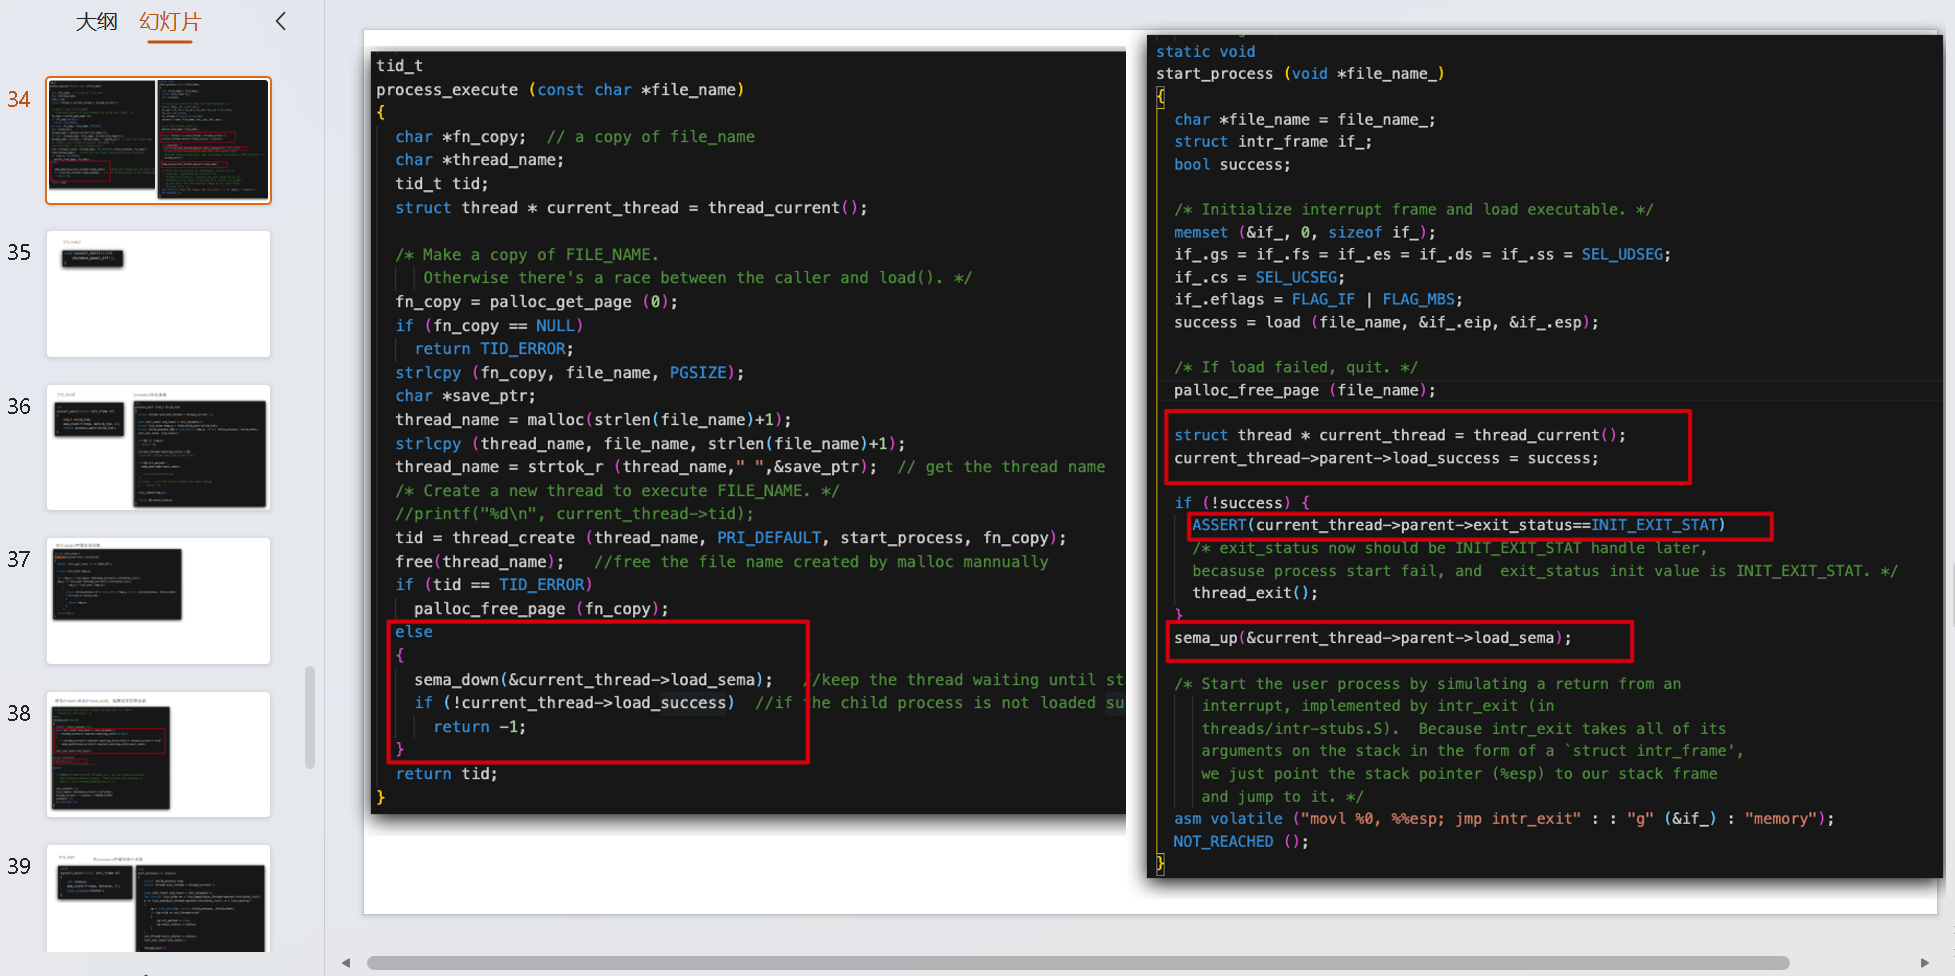
\includegraphics[width=0.85\textwidth]{img6/ale.png}
    \caption{Exec-Ref}
    \label{fig:wait}
\end{figure}

根据以上思路可以在 \texttt{process\_execute()} 函数中加入以下代码:

\begin{lstlisting}[language=C, title = process\_execute()]
    if (tid == TID_ERROR) {
        palloc_free_page (fn_copy);
    } else { 
        sema_down(&current_thread->load_sema);   //让线程一直等待,直到start process()退出。
        if (!current_thread->load_success)  //如果子进程未成功加载
            return -1;   
    }
    return tid;
\end{lstlisting}

另外,我们要在进程启动时,加入 V 操作:

\begin{lstlisting}[language=C, title = start\_process()]
    if (!success) {
        ASSERT(current_thread->parent->exit_status==INIT_EXIT_STAT)
        // 此时 exit_status 应该是稍后的 INIT_EXIT_STAT 句柄
        // 因为进程启动失败,exit_status 初始化值为 INIT_EXIT_STAT
        thread_exit();
      }
      sema_up(&current_thread->parent->load_sema);
\end{lstlisting}

\begin{ctt}
    P 操作 (\texttt{sema\_down}):也称为“等待”操作。当信号量的值大于0时,执行 P 操作会将其减1并继续执行;如果信号量的值为0,线程会阻塞,直到信号量的值大于0。

    V 操作 (\texttt{sema\_up}):也称为“释放”操作。执行 V 操作会将信号量的值加1,并唤醒一个等待该信号量的线程。
\end{ctt}

\begin{rmr}
    当 \texttt{process\_execute()} 调用 \texttt{process\_execute(file\_name)} 创建一个新进程时,新进程的启动过程并非立即完成。子进程需要时间来加载可执行文件、初始化其执行环境等。  
    \texttt{sema\_down(\&current\_thread->load\_sema)} 使得父进程(调用 \texttt{process\_execute()} 的线程)进入等待状态,直到子进程完成加载过程。这确保了父进程在继续执行之前,能够获知子进程是否成功加载。  
    如果子进程在加载过程中失败(例如,可执行文件不存在或格式错误),子进程会通过 \texttt{sema\_up} 操作通知父进程。父进程在被唤醒后,通过检查 \texttt{current\_thread->load\_success} 的值来判断子进程是否成功加载。如果加载失败,父进程返回 \texttt{-1},表示执行失败。

    \vspace{0.5cm}

    无论子进程加载成功还是失败,加载过程结束后都需要通知父进程。\texttt{sema\_up(\&current\_thread->parent->load\_sema)} 执行 V 操作,将信号量的值加1,唤醒等待该信号量的父进程。
    如果子进程加载失败,子进程通过 ASSERT 确认其 \texttt{exit\_status} 被正确初始化为 \texttt{INIT\_EXIT\_STAT},然后调用 \texttt{thread\_exit()} 终止自身。这确保了加载失败的子进程不会继续执行下去。
\end{rmr}

\subsubsection{Wait}

鄙人认为 Exec 和 Wait 的实现很多逻辑上比较相似又比较互补,同样地我们可以从 PPT 中获得一些灵感:

\begin{figure}[H]
    \centering
    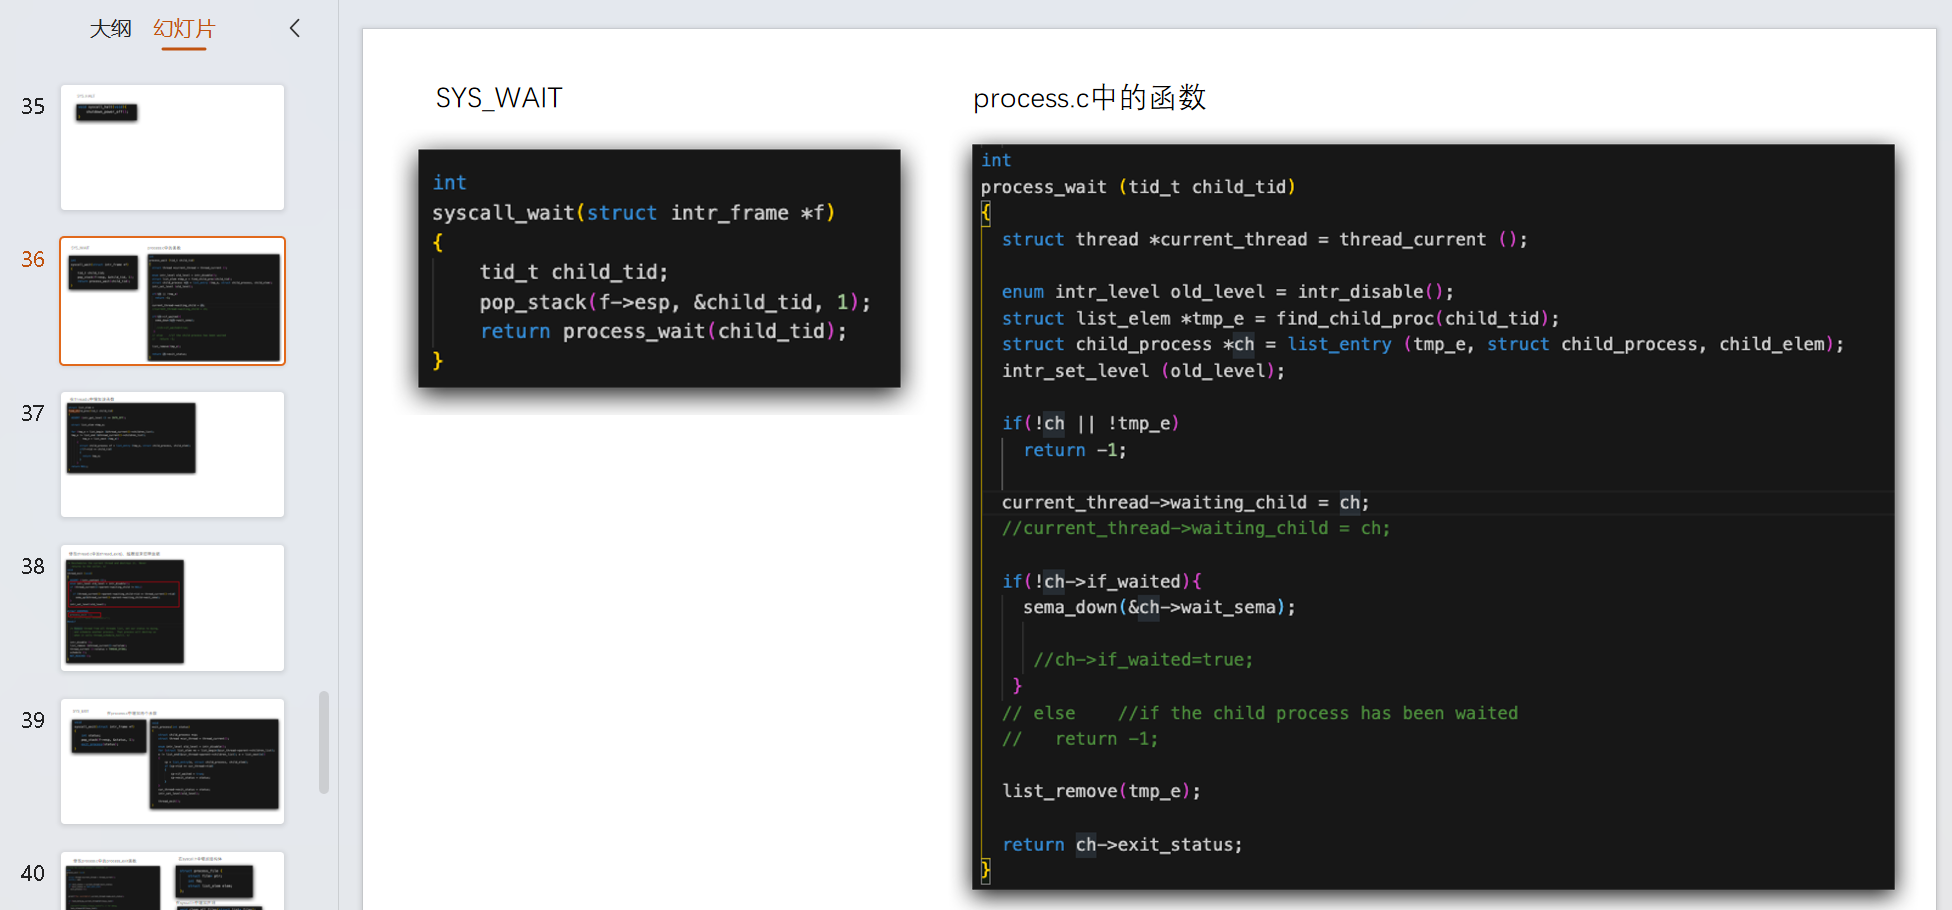
\includegraphics[width=0.8\textwidth]{img6/waitref2.png}
    \caption{Wait-Ref-2}
    \label{fig:wait}
\end{figure}

\begin{mdframed}[backgroundcolor=gray!10, linewidth=0.5pt, roundcorner=5pt]
    当进程系统调用 \texttt{wait} 时,将会等待子进程退出并且返回子进程的 \texttt{pid},取得子进程的退出状态。
\end{mdframed}

\begin{lstlisting}[language=C, title = syscall\_wait()]
    int syscall_wait(struct intr_frame *f) {
        tid_t child_tid;
        pop_stack(f->esp, &child_tid, 1);
        return process_wait(child_tid);
    }
\end{lstlisting}

这段代码很简单,就是从栈中获取 \texttt{child\_tid},然后调用 \texttt{process\_wait()} 函数。

关键在于后面 \texttt{return process\_wait(child\_tid);} 的实现,栈的状态也很清晰:

\begin{lstlisting}
            +----------------+
            | system call ID |  <--- f->esp (栈顶,系统调用号 SYS_WAIT)
            +----------------+
            |   child_tid    |  <--- f->esp + 4 (子进程的线程 ID 参数)
            +----------------+    
\end{lstlisting}

\begin{lstlisting}[language=C, title = process\_wait()]
    int process_wait (tid_t child_tid) {
        /**
        * 等待一个子线程(子进程)的退出,并获取其退出状态。如果子线程尚未退出,当前线程将进入休眠状态,直到子线程退出。
        * 
        * Parameters:child_tid: 子线程的线程 ID
        * Return:
        * - 如果子线程存在并且成功退出,返回其退出状态。
        * - 如果子线程不存在或已经被等待过,返回 -1。
        */
        struct thread *current_thread = thread_current ();

        // 禁用中断,确保对共享资源的安全访问
        enum intr_level old_level = intr_disable();
        struct list_elem *tmp_e = find_child_proc(child_tid); // 在子进程列表中查找子线程对应的链表元素
        struct child_process *ch = list_entry (tmp_e, struct child_process, child_elem); // 提取子线程的状态结构体
        intr_set_level (old_level); // 恢复中断状态

        // 如果子线程不存在,或者对应的链表元素无效,直接返回 -1
        if (!ch || !tmp_e)
            return -1;
    
        // 设置当前线程正在等待的子线程
        current_thread->waiting_child = ch;
    
        // 如果子线程未被等待过,则进入休眠状态,等待子线程退出
        if (!ch->if_waited)
            sema_down(&ch->wait_sema);
    
        // 将子线程从父线程的子进程列表中移除
        list_remove(tmp_e);
    
        // 返回子线程的退出状态
        return ch->exit_status;
}
\end{lstlisting}

\begin{ctt}
    \texttt{process\_wait} 函数用于等待一个子线程(子进程)的退出,并获取其退出状态。
    如果子线程尚未退出,当前线程会通过信号量机制进入休眠,直到子线程退出并唤醒父线程。
    函数首先在子进程列表中查找对应的子线程结构体,检查其合法性,如果合法则阻塞当前线程,
    并在子线程退出后返回其退出状态。如果子线程不存在或已被等待过,函数直接返回 -1。
\end{ctt}

其中用于寻找子进程的函数 \texttt{find\_child\_proc()} 如下(在 \texttt{thread.c} 中定义,然后在 \texttt{thread.h} 中也要包含):

\begin{lstlisting}[language=C, title = find\_child\_proc()]
    struct list_elem *find_child_proc(tid_t child_tid) {
        ASSERT (intr_get_level () == INTR_OFF);
        struct list_elem *tmp_e;
        for (tmp_e = list_begin (&thread_current()->children_list);
             tmp_e != list_end (&thread_current()->children_list);
             tmp_e = list_next (tmp_e)) {
            struct child_process *f = list_entry (tmp_e, struct child_process, child_elem);
                if(f->tid == child_tid) {
                    return tmp_e;
                }
            }
        return NULL;
    }
\end{lstlisting}

在终止时,要释放所有的锁,然后调用 \texttt{clean\_all\_files()} 来关闭开启进程的所有文件。

函数 \texttt{clean\_all\_files} 在 \texttt{syscall.c} 下定义:

\begin{lstlisting}[language=C]
    void clean_all_files(struct list* files) {
        struct process_file *proc_f;
        while(!list_empty(files)) { // 检查文件列表是否为空,如果为空,表示所有的文件已经清理完毕
            proc_f = list_entry (list_pop_front(files), struct process_file, elem);
            file_close(proc_f->ptr);
            list_remove(&proc_f->elem);
            free(proc_f);
        }
    }
\end{lstlisting}

\begin{ctt}
    \begin{itemize}
        \item \texttt{list\_pop\_front(files)}:从链表的前端移除一个元素,并返回该元素的指针。
        
        \item \texttt{list\_entry()}:
        \begin{itemize}
            \item 从链表元素中提取出包含该元素的结构体指针。
            \item 这里提取的结构体是 \texttt{struct process\_file},存储在 \texttt{proc\_f} 中。
        \end{itemize}
        
        \item \texttt{file\_close(proc\_f->ptr)}:
        \begin{itemize}
            \item 调用文件系统的 \texttt{file\_close} 函数,关闭当前文件指针 \texttt{proc\_f->ptr}。
            \item 这是资源清理的关键步骤,确保文件被正确关闭,释放内核资源。
        \end{itemize}
        
        \item \texttt{list\_remove(\&proc\_f->elem)}:从链表中移除 \texttt{proc\_f} 对应的链表节点。防止链表中遗留无效的节点。
    \end{itemize}
\end{ctt}

注意我们要在 \texttt{syscall.h} 中定义一个新的数据结构,以辅助这个函数的实现:

\begin{lstlisting}[language=C]
    struct process_file {
        struct file *ptr;           // 指向打开的文件
        int fd;                     // 文件描述符
        struct list_elem elem;      // 链表节点,用于将该结构体加入链表
    };    
\end{lstlisting}



\subsubsection{阶段性 Make Check}

在上一次为了实现部分系统调用时,我们已经实现了 \texttt{syscall\_write()} 函数。

我们根据上一次的框架来进行一次测试,看看目前可以通过多少测试点:

\begin{center}
\begin{figure}[H]
    \centering
    \begin{subfigure}[b]{0.35\textwidth}
        \centering
        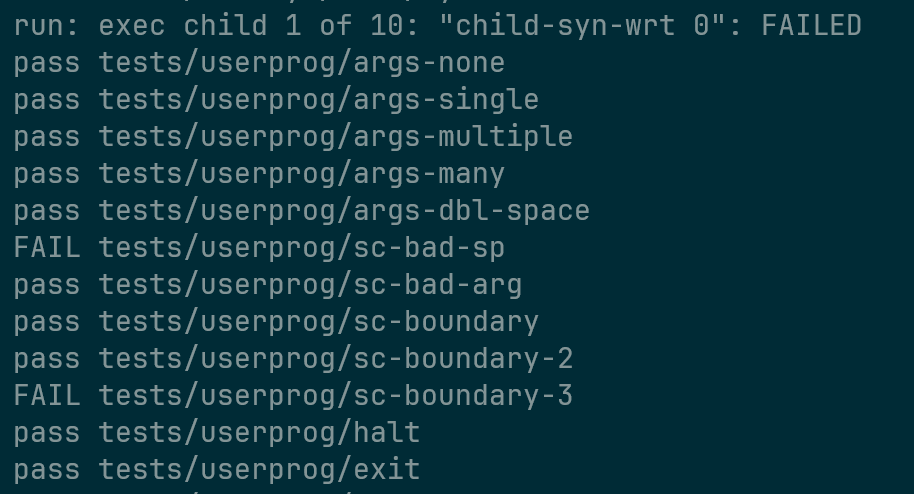
\includegraphics[width=\textwidth]{img6/passpart1.png}
        \caption{参数传递和 Exit、Halt}
        \label{fig:part1}
    \end{subfigure}
    \hspace{1cm}
    \begin{subfigure}[b]{0.35\textwidth}
        \centering
        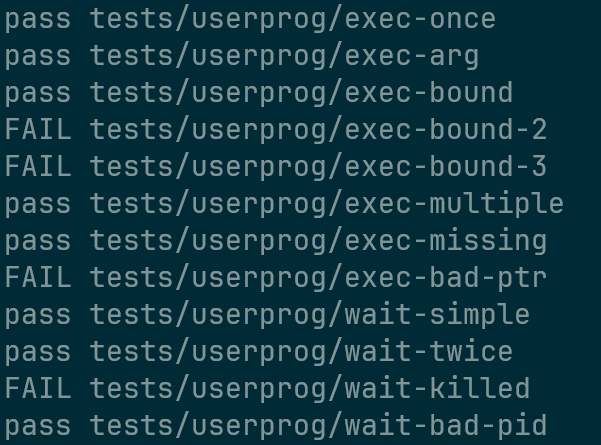
\includegraphics[width=\textwidth]{img6/passpart2.png}
        \caption{Exec 和 Wait}
        \label{fig:part2}
    \end{subfigure}
    \caption{Part 1 and Part 2}
    \label{fig:test}
\end{figure}
\end{center}

此时显示刚好有一半的测试点是通过的,具体不知道为什么有一些和 Exec 有关的测试点没有通过。

我猜测可能要结合后面和文件相关吧,所以我们这里先告一段落了,后面有 BUG 再回来修。

\begin{figure}[H]
    \centering
    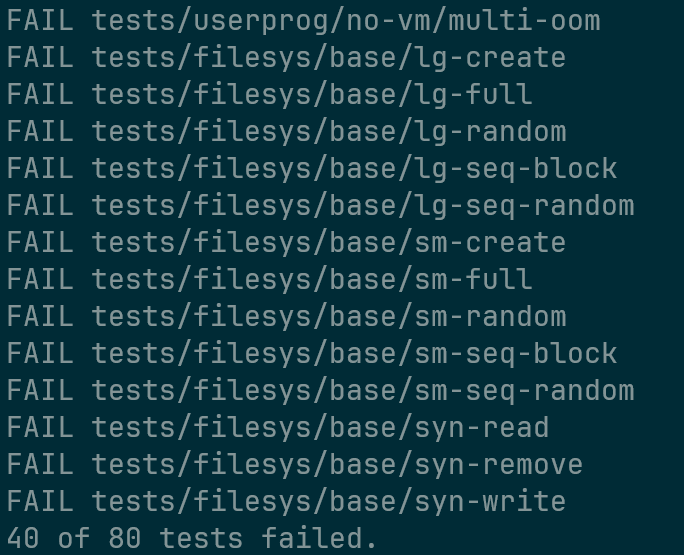
\includegraphics[width=0.38\textwidth]{img6/passhalf.png}
    \caption{Half Passed}
    \label{fig:part3}
\end{figure}

可以看到,当我们把进程有关的所有系统调用都实现后,已经可以通过很大一部分的检查点了。
接下来,我们就要进入文件相关的部分了。

\subsubsection{进入文件部分}

接下来我们进入的就是 Pintos 中和文件管理相关的部分了。

之前定义的数据结构中,有一部分就是用于文件操作的:

\begin{figure}[H]
    \centering
    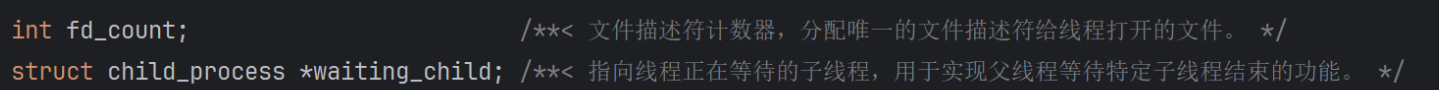
\includegraphics[width=0.935\textwidth]{img6/new.png}
    \caption{File Data Structure}
    \label{fig:file}
\end{figure}
    
为了维护每个进程打开了的文件列表,统计每个进程打开了的文件数目,

\texttt{syscall\_write} 已经在上一次实验中实现了,但是由于有跳步的情况,在这里重新拿过来做一下分析:

\begin{rmr}
Pintos 中已经为我们实现了文件系统,并且给我们提供了部分接口来使用,在官方文档中有提到:
\end{rmr}

\begin{figure}[H]
    \centering
    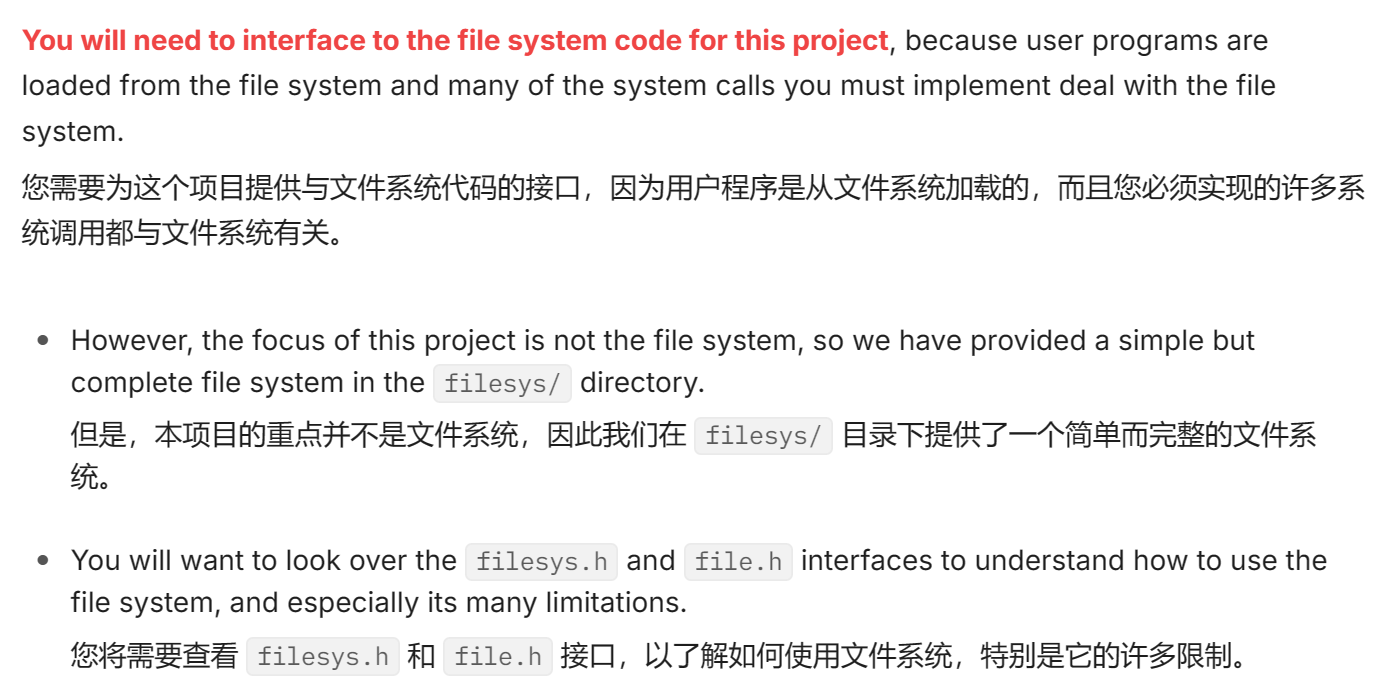
\includegraphics[width=0.62\textwidth]{img6/API.png}
    \caption{File System Doc}
    \label{fig:fsdoc}
\end{figure}

在 PPT 中也有所总结:

\begin{figure}[H]
    \centering
    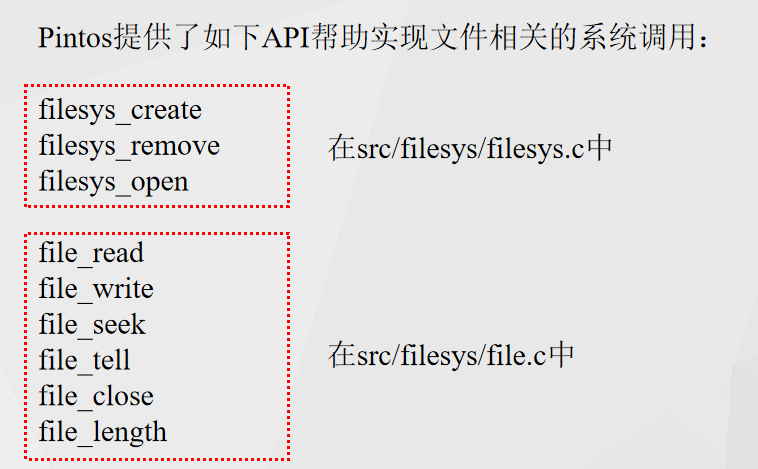
\includegraphics[width=0.35\textwidth]{img6/apippt.png}
    \caption{File System API}
    \label{fig:fs}
\end{figure}

另外需要注意的是,Pintos 中一次只能执行一个文件,在官方文档中提到:Pintos 暂未实现内部同步,并发的访问会相互干扰。

\begin{figure}[H]
    \centering
    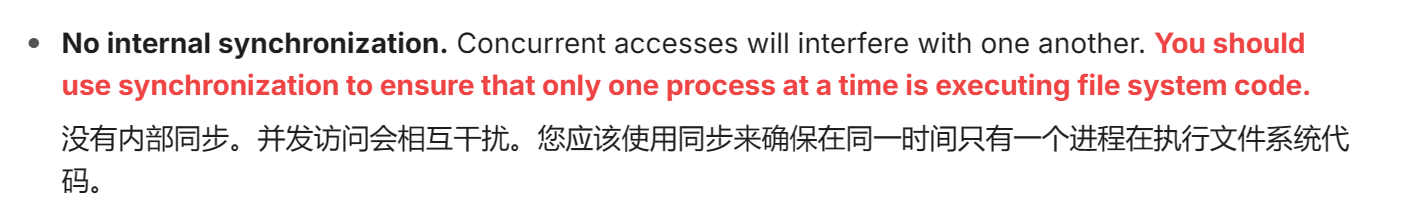
\includegraphics[width=0.67\textwidth]{img6/nosyn.png}
    \caption{File System No Sync}
    \label{fig:sync}
\end{figure}

还有一份 PPT 中的内容多了一个数据 \texttt{struct list opened\_files},根据名字可见它的作用,那么我们也把它添加到 \texttt{thread.h} 中,然后完成这一份系统调用。

按照提示,我们继续把文件锁添加到 \texttt{thread.h} 中,最后,为了处理临界区问题,我们可以在 \texttt{load} 的临界区进入前后加入一个对 \texttt{filesys\_lock} 锁的申请。

\begin{lstlisting}[language=C]
    lock_acquire(&filesys_lock); // 获取文件系统全局锁,以防止并发访问文件系统时发生数据竞争
    ret = filesys_create(name, initial_size); // 调用文件系统的创建函数,它的返回值为 bool
    lock_release(&filesys_lock); // 释放文件系统锁,允许其他线程访问文件系统
\end{lstlisting}

现在,我们可以通过 Pintos 提供的接口来逐步实现这些系统调用了。

\subsubsection{Write}

\begin{lstlisting}[language=C, title= syscall\_write()]
    int syscall_write(struct intr_frame *f) {
        int ret;                  /**< 写入操作的返回值。 */
        int size;                 /**< 要写入的数据大小(字节)。 */
        void *buffer;             /**< 数据缓冲区的起始地址。 */
        int fd;                   /**< 文件描述符。 */
    
        // 从用户栈中读取系统调用参数,分别是 size、buffer 和 fd
        pop_stack(f->esp, &size, 7);
        pop_stack(f->esp, &buffer, 6);
        pop_stack(f->esp, &fd, 5);
    
        // 检查 buffer 是否为有效的用户地址
        if (!is_valid_addr(buffer))
            ret = -1;

        // 如果文件描述符是标准输出(fd == 1),直接将数据输出到控制台
        if (fd == 1) {
            putbuf(buffer, size); /**< 调用系统提供的 putbuf() 函数写入控制台。 */
            ret = size;           /**< 返回写入的字节数,即 size。 */
        } else {
            // 文件写入操作,需要查找文件描述符对应的文件指针
            enum intr_level old_level = intr_disable(); /**< 禁用中断,避免多线程竞争。 */
            struct process_file *pf = search_fd(&thread_current()->opened_files, fd);
            intr_set_level(old_level); /**< 恢复中断状态。 */
            // 如果文件描述符无效,返回错误
            if (pf == NULL) ret = -1;
            else {
                // 获取文件系统锁,确保文件写操作是线程安全的
                lock_acquire(&filesys_lock);
                ret = file_write(pf->ptr, buffer, size); /**< 写入数据到文件,返回写入字节数。 */
                lock_release(&filesys_lock);
            }
        }
        return ret;
    }
\end{lstlisting}

\begin{ctt}

\texttt{syscall\_write} 函数实现了系统调用,用于向文件或标准输出写入数据。
函数首先通过从用户栈中读取参数(\texttt{size、buffer、fd})完成参数传递,确保用户态与内核态的隔离。
随后,检查缓冲区地址是否为有效的用户地址,以防止非法内存访问,保护操作系统的安全性。
如果文件描述符为标准输出(\texttt{fd == 1}),直接调用 \texttt{putbuf} 将数据输出到控制台,绕过文件系统以提高效率。

\vspace{0.5cm}

对于其他文件描述符,函数通过禁用中断和文件系统锁保证线程安全,
查询文件描述符对应的文件指针并执行文件写入操作,同时确保多线程环境下的资源管理。

\end{ctt}

\subsubsection{Create}

接下来我们进入第二个文件系统调用,\texttt{create()}:

在 Pintos Guide 上它的定义如下:

\begin{figure}[H]
    \centering
    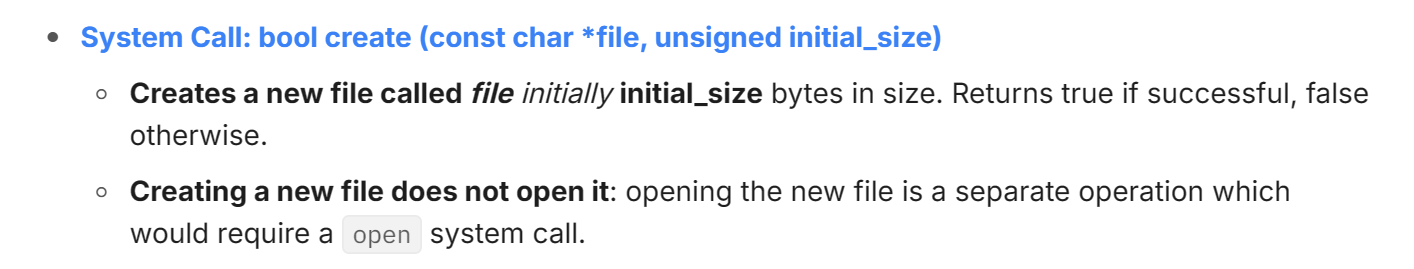
\includegraphics[width=0.7\textwidth]{img6/createdoc.png}
    \caption{Create Doc}
    \label{fig:create}
\end{figure}

幸运的是,PPT 中已经给了我们实现的逻辑,还记得图 \ref{fig:check} 吗?但是 PPT 里的函数有一点小问题。

我们可以直接拿过来修修补补直接用:

\begin{figure}[H]
    \centering
    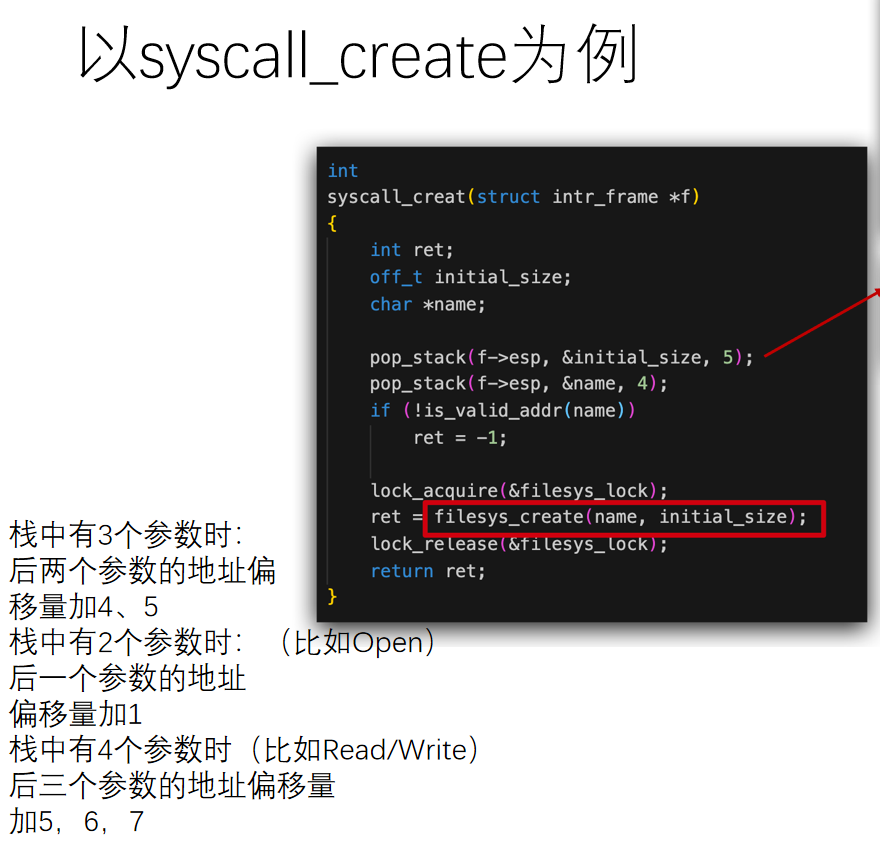
\includegraphics[width=0.3\textwidth]{img6/fix.png}
    \caption{Create}
    \label{fig:create_fix}
\end{figure}

之后就是喜闻乐见的沿用 PPT 上的例子并进行分析了:

\begin{lstlisting}[language=C, title= syscall\_create()]
    void syscall_create(struct intr_frame *f) {
        int ret;
        off_t initial_size;
        char *name;
    
        pop_stack(f->esp, &initial_size, 5);
        pop_stack(f->esp, &name, 4);
        if (!is_valid_addr(name))
            ret = -1;
    
        lock_acquire(&filesys_lock); // 获取文件系统全局锁,以防止并发访问文件系统时发生数据竞争
        ret = filesys_create(name, initial_size); // 调用文件系统的创建函数,它的返回值为 bool
        lock_release(&filesys_lock); // 释放文件系统锁,允许其他线程访问文件系统
        return ret;
    }
\end{lstlisting}

至于为什么在 \texttt{pop\_stack()} 函数里写 $4, 5$,是因为:

\begin{figure}[H]
    \centering
    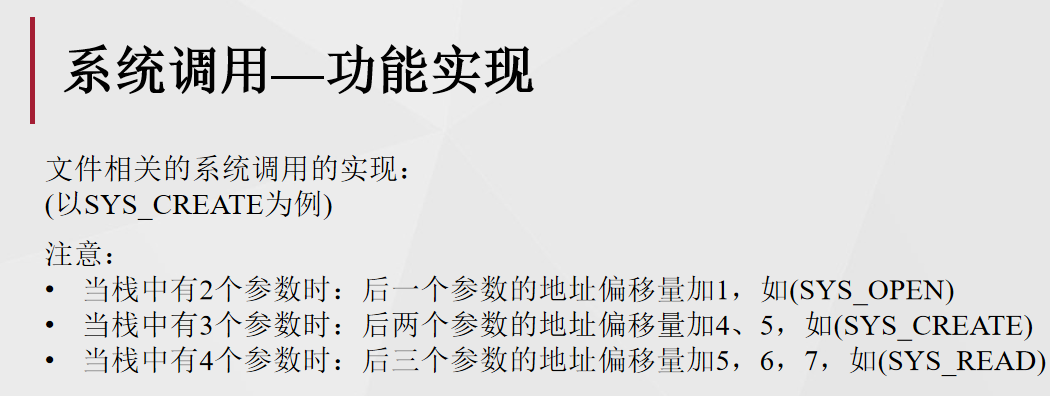
\includegraphics[width=0.5\textwidth]{img6/number.png}
    \caption{Stack}
    \label{fig:stack}
\end{figure}

\begin{itemize}
    \item 当栈中有 \textbf{2个参数} 时:后一个参数的地址偏移量加1,例如(\texttt{SYS\_OPEN})。
    \item 当栈中有 \textbf{3个参数} 时:后两个参数的地址偏移量加4、5,例如(\texttt{SYS\_CREATE})。
    \item 当栈中有 \textbf{4个参数} 时:后三个参数的地址偏移量加5、6、7,例如(\texttt{SYS\_READ})。
\end{itemize}

此时的栈结构如下所示,这是 \texttt{pop\_stack()} 调用的由来。

\begin{lstlisting}
            +----------------+
            | system call ID | <--- f->esp (create 的系统调用号)
            +----------------+
            |   name (指针)  | <--- f->esp + 4
            +----------------+
            | initial_size   | <--- f->esp + 8
            +----------------+    
\end{lstlisting}

\subsubsection{Remove}

当实现了上面最难的部分的系统调用后,其他的就很简单了。现在我们来实现 Remove.

\begin{lstlisting}[language=C, title= syscall\_remove()]
    /**
    * 功能: 从栈中提取文件名参数,检查文件名地址的合法性。调用文件系统接口 filesys_remove() 删除文件。
    *       无论文件是否被打开,都可以成功删除,但文件删除后并不会自动关闭文件句柄。
    * Parameters:
    *    struct intr_frame *f: 系统调用中断帧,用于获取用户栈上的参数。
    * 
    * Return:
    * - 成功时返回 1 (true),表示文件删除成功。
    * - 失败时返回 -1 或 0 (false),表示删除失败。
    */
   int syscall_remove(struct intr_frame *f) {
       int ret;
       char *name;      

       pop_stack(f->esp, &name, 1); // 从用户栈中提取文件名参数
       if (!is_valid_addr(name)) // 检查文件名的地址是否合法
           ret = -1;
   
       // 加锁,确保文件系统操作的线程安全
       lock_acquire(&filesys_lock);
   
       if (filesys_remove(name) == NULL) 
           ret = false;
       else 
           ret = true;
   
       // 释放文件系统锁
       lock_release(&filesys_lock);
       return ret;
   }
\end{lstlisting}

有了之前对于上锁的分析后,这部分实现起来完全就没有难度了,毕竟已经给好了接口了。

\subsubsection{Open}

要求如文档所示:

\begin{figure}[H]
    \centering
    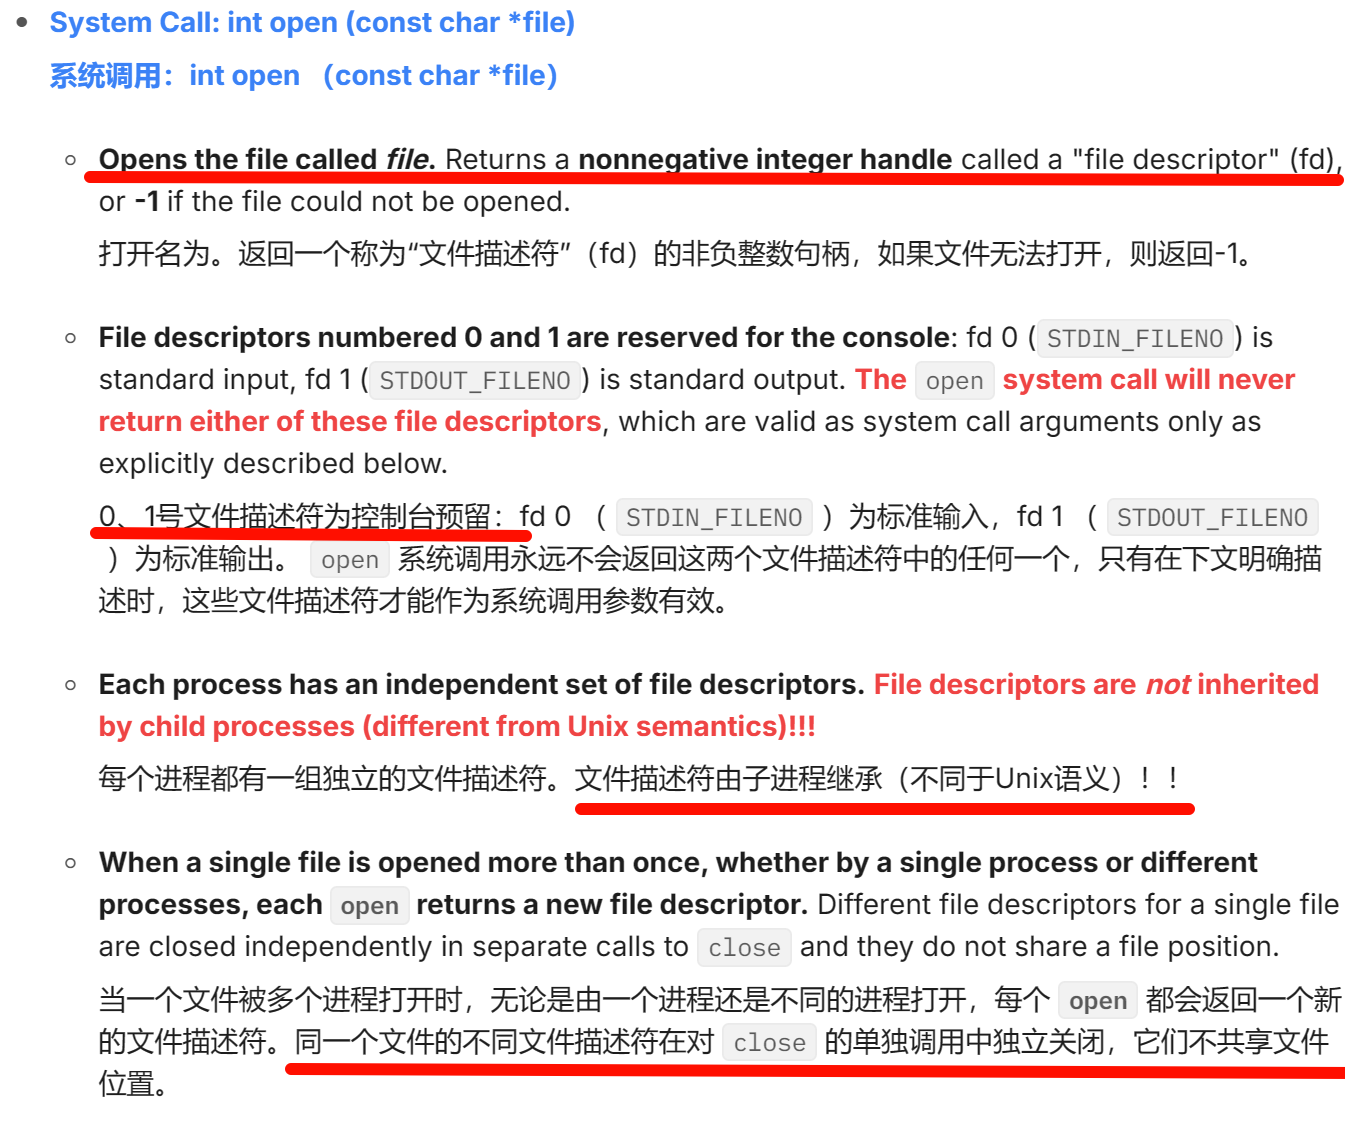
\includegraphics[width=0.53\textwidth]{img6/opendoc.png}
    \caption{Open Doc}
    \label{fig:open}
\end{figure}

根据提示,我们应该要在保证互斥的情况下调用 \texttt{filesys\_open()},
将取得的文件和文件指针存储到 \texttt{struct process\_file} 中,
然后将其加入 \texttt{thread\_current()->opened\_files} 链表。

\begin{lstlisting}[language=C, title= syscall\_open()]
    int syscall_open(struct intr_frame *f) {
        int ret;
        char *name;
    
        // 从用户栈中读取系统调用参数,即文件名
        pop_stack(f->esp, &name, 1);
    
        // 检查文件名地址是否合法以及文件名长度是否大于零
        if (!is_valid_addr(name) || strlen(name) == 0){
            ret = -1;
            return ret;
        }
    
        // 获取文件系统锁,确保文件系统操作的线程安全
        lock_acquire(&filesys_lock);
        struct file *fptr = filesys_open(name); /**< 调用文件系统的打开函数,返回文件指针。 */
        lock_release(&filesys_lock); /**< 释放文件系统锁 */
    
        // 如果文件不存在,返回 -1
        if (fptr == NULL)
            ret = -1;
        else {
            // 分配并初始化新的 process_file 结构体
            struct process_file *pfile = malloc(sizeof(*pfile));
            pfile->ptr = fptr; /**< 文件指针赋值 */
            pfile->fd = thread_current()->fd_count; /**< 分配新的文件描述符 */
            thread_current()->fd_count++; /**< 文件描述符计数器递增 */
            list_push_back(&thread_current()->opened_files, &pfile->elem); /**< 将文件加入当前线程的打开文件列表 */
            ret = pfile->fd; /**< 返回文件描述符 */
        }
        return ret;
    }
\end{lstlisting}
    
\begin{cth}
    
    \texttt{syscall\_open} 实现了用户程序通过系统调用打开指定文件的功能。函数首先从用户栈中获取 \texttt{name} 参数,确保参数传递的正确性。
    
    1. 调用 \texttt{is\_valid\_addr(name)} 函数,检查文件名指针的合法性,防止用户程序传入非法地址。
    2. 检查文件名长度是否大于零,避免打开空文件名的情况。
    
    \vspace{0.3cm}

    在确认文件名地址合法且非空后,获取全局文件系统锁 \texttt{filesys\_lock},确保文件系统操作的线程安全。调用 \texttt{filesys\_open(name)} 函数尝试打开指定文件,并根据返回值判断文件是否存在:

    \begin{itemize}
        \item 如果文件不存在(\texttt{fptr == NULL}),返回 \texttt{-1}。
        \item 如果文件存在,分配并初始化新的 \texttt{struct process\_file} 结构体,将文件指针和分配的文件描述符存储其中,并将该结构体加入当前线程的打开文件列表 \texttt{opened\_files} 中。
    \end{itemize}
    
\end{cth}

\subsubsection{Filesize}

返回文件的大小。

\begin{lstlisting}[language=C, title= syscall\_filesize()]
    int syscall_filesize(struct intr_frame *f) {
        int ret; 
        int fd;
        
        // 从用户栈中读取系统调用参数,即文件描述符
        pop_stack(f->esp, &fd, 1);
        
        // 获取文件系统锁,确保文件系统操作的线程安全
        lock_acquire(&filesys_lock);
        
        // 查找文件描述符对应的文件指针,并获取文件大小
        struct process_file *pf = search_fd(&thread_current()->opened_files, fd);
        if (pf == NULL) {
            ret = -1; 
        } else {
            ret = file_length(pf->ptr); 
        }
        
        // 释放文件系统锁
        lock_release(&filesys_lock);
        
        return ret; 
    }
\end{lstlisting}
    
\begin{ctt}
    \texttt{syscall\_filesize} 实现了用户程序通过系统调用获取指定文件大小的功能。函数首先从用户栈中获取 \texttt{fd} 参数,确保参数传递的正确性。
    调用 \texttt{search\_fd} 函数,根据文件描述符 \texttt{fd} 查找对应的 \texttt{struct process\_file} 结构体。如果查找失败(即 \texttt{pf == NULL}),则返回 \texttt{-1},表示文件描述符无效。
    在确认有效后,调用 \texttt{file\_length(pf->ptr)} 函数获取文件的字节大小,并将其赋值给 \texttt{ret}。
\end{ctt}

其中,子函数 \texttt{search\_fd()} 用于根据文件描述符返回一个 \texttt{process\_file} 的结构体,
可以用这个结构体来获取到文件的内存地址。函数实现如下所示:

\begin{lstlisting}[language=C, title= search\_fd()]
    struct process_file *search_fd(struct list* files, int fd) {
        struct process_file *proc_f;
        for (struct list_elem *e = list_begin(files); e != list_end(files); e = list_next(e)) {
            proc_f = list_entry(e, struct process_file, elem);
            if (proc_f->fd == fd)
                return proc_f;
        }
        return NULL;
    }
\end{lstlisting}

\subsubsection{Read}

根据文件描述符 fd 将制定的 size 字节数据读入到缓存当中,返回实际读取到的字节数
或者 -1 (当文件无法读取的时候)

\begin{lstlisting}[language=C, title= syscall\_read()]
    int syscall_read(struct intr_frame *f) {
        int ret;             /**< 读取操作的返回值,即实际读取的字节数。 */
        int size;            /**< 要读取的数据大小(字节)。 */
        void *buffer;        /**< 数据缓冲区的起始地址。 */
        int fd;              /**< 文件描述符。 */
    
        // 从用户栈中读取系统调用参数,分别是 size、buffer 和 fd
        pop_stack(f->esp, &size, 7);
        pop_stack(f->esp, &buffer, 6);
        pop_stack(f->esp, &fd, 5);
    
        // 检查 buffer 是否为有效的用户地址
        if (!is_valid_addr(buffer)) {
            ret = -1; /**< 地址无效,返回错误码。 */
        }
    
        // 如果文件描述符是标准输入(fd == 0),从输入缓冲区读取数据
        if (fd == 0) {
            int i;
            uint8_t *buf = buffer;
            for (i = 0; i < size; i++)
                buf[i] = input_getc(); /**< 从键盘读取一个字符。 */
            ret = size; /**< 返回读取的字节数。 */
        } else {
            // 文件读取操作,需要查找文件描述符对应的文件指针
            struct process_file *pf = search_fd(&thread_current()->opened_files, fd);
            if (pf == NULL)
                ret = -1; /**< 文件描述符无效,返回错误码。 */
            else {
                // 获取文件系统锁,确保文件读取操作的线程安全
                lock_acquire(&filesys_lock);
                ret = file_read(pf->ptr, buffer, size); /**< 从文件中读取数据,返回实际读取的字节数。 */
                lock_release(&filesys_lock);
            }
        }
        return ret; /**< 返回读取的字节数或错误码。 */
    }
    \end{lstlisting}
    
    \begin{cth}
    
    \texttt{syscall\_read} 实现了用户程序通过系统调用从文件或标准输入读取数据的功能。函数首先从用户栈中获取 \texttt{size}、\texttt{buffer} 和 \texttt{fd} 这三个参数,确保参数传递的正确性。
    
    在确认文件描述符有效后,获取全局文件系统锁 \texttt{filesys\_lock},确保文件读取操作的线程安全。调用 \texttt{file\_read} 函数执行实际的文件读取操作,并将读取到的字节数赋值给 \texttt{ret}。
    根据读取操作的结果,返回实际读取的字节数。如果任何步骤中出现错误,返回 \texttt{-1} 以指示读取失败。
    \end{cth}

\subsubsection{Seek}

查找调用,即改变下一个要进行读/写的字节位置。
当读的位置超过了 EOF 时不能报错,而是读取到字节,以表示已经到达了文件结尾。
而写的操作超过了 EOF时将会抛出错误。(由 \texttt{file\_seek()} 已经实现)

\begin{lstlisting}[language=C, title= syscall\_seek()]
    void syscall_seek(struct intr_frame *f) {
        int fd;  /**< 文件描述符。 */
        int pos; /**< 新的文件指针位置。 */
    
        // 从用户栈中读取系统调用参数,分别是 pos 和 fd
        pop_stack(f->esp, &fd, 5);
        pop_stack(f->esp, &pos, 4);
    
        // 查找文件描述符对应的文件指针
        struct process_file *pf = search_fd(&thread_current()->opened_files, fd);
        if (pf == NULL) {
            // 如果文件描述符无效,调用 exit 退出进程
            exit_process(-1);
        }
    
        // 获取文件系统锁,确保文件操作的线程安全
        lock_acquire(&filesys_lock);
        file_seek(pf->ptr, pos); /**< 调整文件指针的位置。 */
        lock_release(&filesys_lock);
    }
    \end{lstlisting}
    
    \begin{ctt}
    \texttt{syscall\_seek} 实现了用户程序通过系统调用调整文件指针位置的功能。函数首先从用户栈中获取 \texttt{fd} 和 \texttt{pos} 这两个参数,确保参数传递的正确性。
    
    调用 \texttt{search\_fd} 函数,根据文件描述符 \texttt{fd} 查找对应的 \texttt{struct process\_file} 结构体。如果查找失败(即 \texttt{pf == NULL}),则调用 \texttt{exit\_process(-1)} 终止当前进程,以指示非法文件描述符的使用。
    
    在确认文件描述符有效后,获取全局文件系统锁 \texttt{filesys\_lock},确保文件操作的线程安全。调用 \texttt{file\_seek(pf->ptr, pos)} 函数调整文件指针的位置到指定的 \texttt{pos}。
    \end{ctt}

\subsubsection{Tell}

取得文件的读取位置,返回值是下一个将被读取或者写入的字节位置。

\begin{lstlisting}[language=C]
    int syscall_tell(struct intr_frame *f) {
        int ret; /**< 文件指针位置的返回值。 */
        int fd;  /**< 文件描述符。 */
    
        // 从用户栈中读取系统调用参数,即文件描述符
        pop_stack(f->esp, &fd, 1);
    
        // 查找文件描述符对应的文件指针
        struct process_file *pf = search_fd(&thread_current()->opened_files, fd);
        if (pf == NULL) {
            ret = -1; /**< 如果文件描述符无效,返回 -1。 */
        } else {
            // 获取文件系统锁,确保文件操作的线程安全
            lock_acquire(&filesys_lock);
            ret = file_tell(pf->ptr); /**< 获取当前文件指针的位置。 */
            lock_release(&filesys_lock);
        }
    
        return ret; /**< 返回文件指针的位置或错误码。 */
    }
    \end{lstlisting}
    
    \begin{cth}
    \texttt{syscall\_tell} 实现了用户程序通过系统调用获取当前文件指针位置的功能。函数首先从用户栈中获取 \texttt{fd} 参数,确保参数传递的正确性。
    
    调用 \texttt{search\_fd} 函数,根据文件描述符 \texttt{fd} 查找对应的 \texttt{struct process\_file} 结构体。如果查找失败(即 \texttt{pf == NULL}),则返回 \texttt{-1},表示文件描述符无效。
    
    在确认文件描述符有效后,获取全局文件系统锁 \texttt{filesys\_lock},确保文件操作的线程安全。调用 \texttt{file\_tell(pf->ptr)} 函数获取当前文件指针的位置,并将其赋值给 \texttt{ret}。
    \end{cth}

\subsubsection{Close}

最后一个系统调用是实现文件的关闭操作,这个调用将会在任意进程中止的时候依次调用。

\begin{lstlisting}[language=C]
    void syscall_close(struct intr_frame *f) {
        int fd;
    
        // 从用户栈中读取系统调用参数,即文件描述符
        pop_stack(f->esp, &fd, 1);
    
        // 检查文件描述符是否为标准输入(fd == 0)或标准输出(fd == 1)
        if(fd == 1 || fd == 0){
            exit_process(-1); 
        }
    
        // 查找文件描述符对应的文件指针
        struct process_file *pf = search_fd(&thread_current()->opened_files, fd);
        if (pf == NULL) {
            exit_process(-1);
        }
    
        // 获取文件系统锁,确保文件操作的线程安全
        lock_acquire(&filesys_lock);
        clean_single_file(&thread_current()->opened_files, fd); /**< 关闭并清理指定的文件。 */
        lock_release(&filesys_lock);
    }
    \end{lstlisting}
    
\begin{ctt}
    \texttt{syscall\_close} 实现了用户程序通过系统调用关闭指定文件的功能。函数首先从用户栈中获取 \texttt{fd} 参数,确保参数传递的正确性。
    由于 \texttt{close} 操作不需要向用户程序返回值,因此函数类型为 \texttt{void}。
\end{ctt}

嵌套的子函数用于关闭一个指定的文件(\texttt{clean\_single\_file()}),这时候不需要再重复用文件单锁来处理互斥问题:

\begin{lstlisting}[language=C]
    void clean_single_file(struct list* files, int fd) {
        struct process_file *proc_f = search_fd(files,fd);
        if (proc_f != NULL){
            file_close(proc_f->ptr);
            list_remove(&proc_f->elem);
            free(proc_f);
        }
    }
\end{lstlisting}

\subsection{Mission 5: Denying Writes to Executables}

最后一个任务是要求不能允许进程写正在执行的进程文件。

\begin{figure}[H]
    \centering
    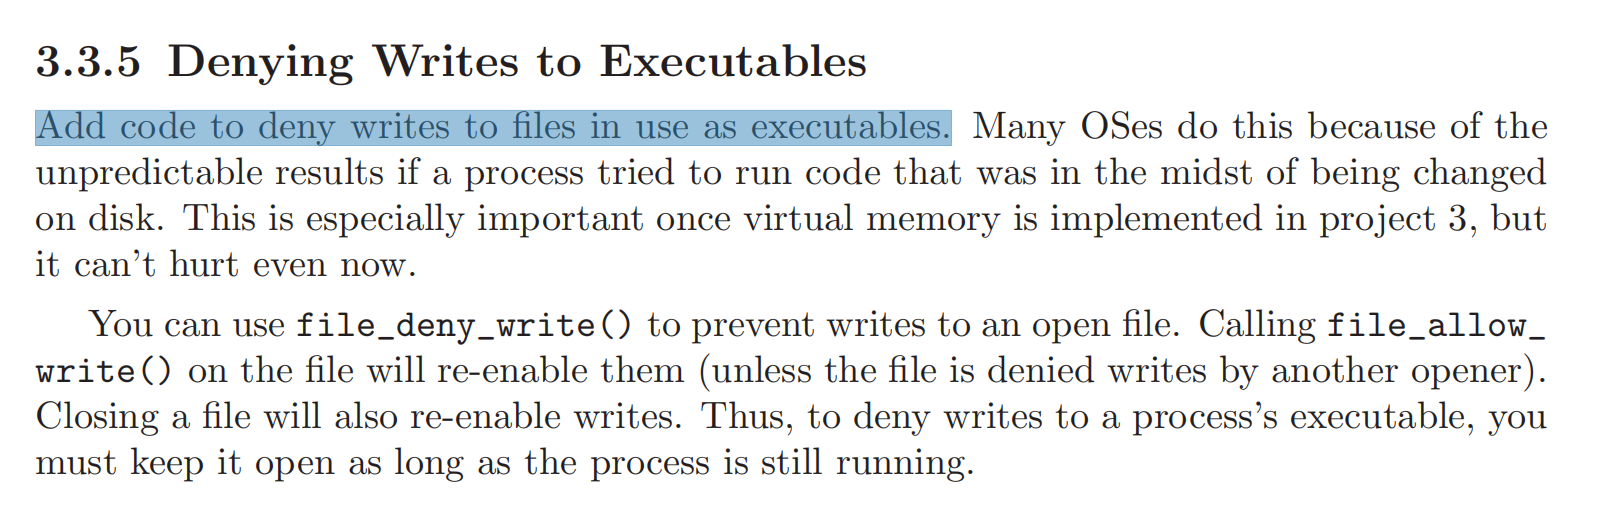
\includegraphics[width=0.57\textwidth]{img6/denying.png}
    \caption{Denying Writes to Executables}
    \label{fig:deny_writes}
\end{figure}

在官方文档中提到,在进程创建时,只需要调用 \texttt{file\_deny\_write()} 使该文件无法被写,
在进程结束的时候调用 \texttt{file\_allow\_write()} 使该文件重新允许被写即可。

这两个文件在 \texttt{filesys.c} 中已经有定义:

\begin{figure}[H]
    \centering
    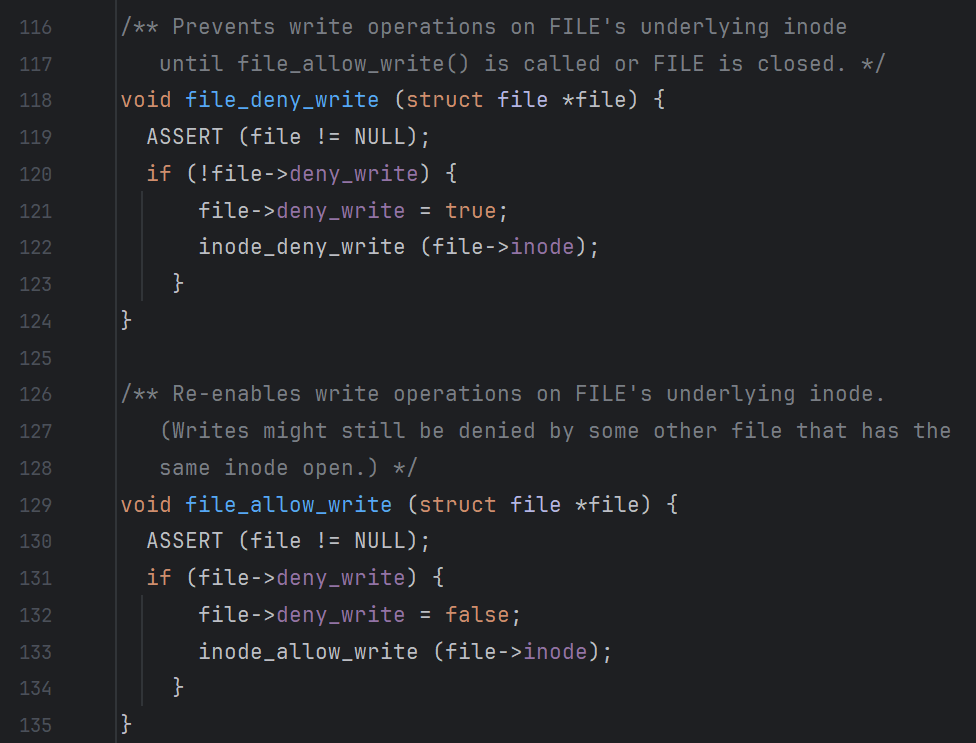
\includegraphics[width=0.52\textwidth]{img6/denyandwrite.png}
    \caption{file\_deny\_write() and file\_allow\_write()}
    \label{fig:deny_writes_code}
\end{figure}

这一部分就较为简单了,毕竟已经实现了接口了,我们只需要在 \texttt{process.c} 的 \texttt{load} 函数中加入语句:

\begin{lstlisting}[language=C]
    file_deny_write(file);
\end{lstlisting}

这样就禁止了其他进程对该正在运行的文件进行写操作。然后只需要在进程退出时再允许写就好啦:

\begin{lstlisting}[language=C, title = exit\_process()]
    file_allow_write(current_thread->self);
\end{lstlisting}

到此为止,我们已经完成了 Pintos Project - Userprog 的全部内容。

\section{实验结果}

在经历了 Project 2 的九九八十一难之后,我们终于获得了最后悦动的 All Passed!

\begin{figure}[H]
    \centering
    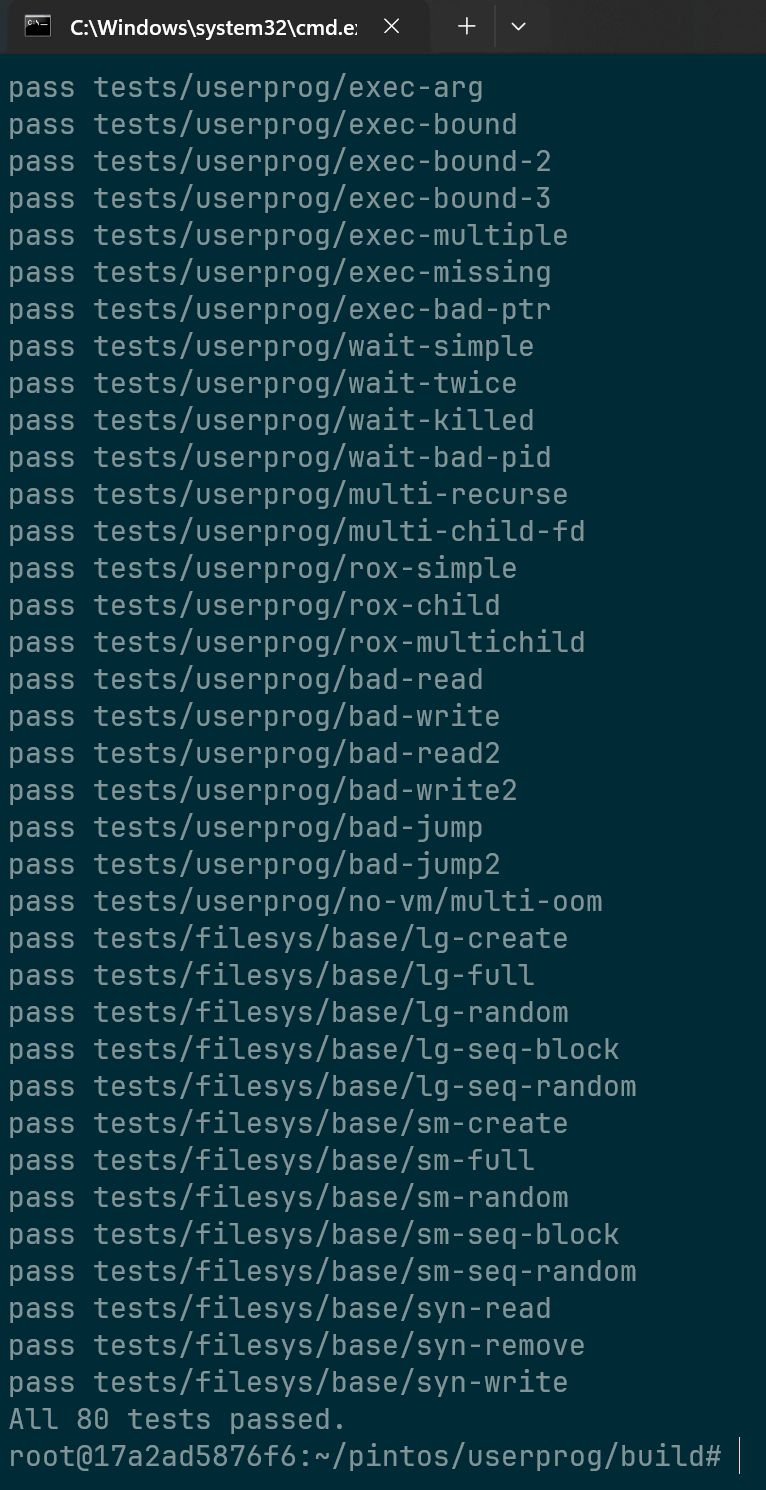
\includegraphics[width=0.23\textwidth]{img6/allpass.png}
    \caption{All Passed}
    \label{fig:all_passed}
\end{figure}

我决定在 LateX 中把这张图片直接放成长图,因为它确实值得这个长度!

\vspace{0.4cm}

\begin{proof}

这一定是我在实验中最最有成就感的一次,必须得夸 Pintos 的设计之精美,像当年在 Minecraft 中研究红石那般有趣。
不断地分析问题,不断地搜索问题,解决问题。
写报告的每一步,用上一个成语的瞬间,都觉得自己在修炼一个屠龙之术,在解决一个 Project 后才深刻明白,
自己的所侍之才不过是雕虫小技罢了。

\vspace{0.5cm}

不过,书写的过程也愈发觉得自己的菜,
查阅了非常多的中文毒瘤 CSDN 的资料,也在 Github 上辗转多处,
只为找到一个最优解,Bing 的国际版历史记录也全是各种 Pintos Userprog 等关键词。
或许捣鼓都是值得的,两千多行的 LateX 代码也是肝的见证。
\end{proof}

其中的一个测试点 multi-oom 非常给力,前两次测试无法通过,显示 \textbf{1 of 80 tests failed},查阅资料后发现:

\begin{figure}[H]
    \centering
    
\includegraphics[width=0.8\textwidth]{img6/multioom.png}
    \caption{UTEXAS For Pintos}
    \label{fig:multi_oom}
\end{figure}

就连 UTEXAS(得克萨斯大学奥斯汀分校)的官方文档也提到:

\begin{mdframed}
    除了这个测试点之外,其他都过了,就可以进入 Project 3!可以看出它到底有多折磨人。
\end{mdframed}

为了查一个究竟,我在知乎上找到了一篇文章介绍了 \texttt{Multi-oom} 的工作原理:\href{https://zhuanlan.zhihu.com/p/340428650}{\underline{https://zhuanlan.zhihu.com/p/340428650}}

\begin{figure}[H]
    \centering
    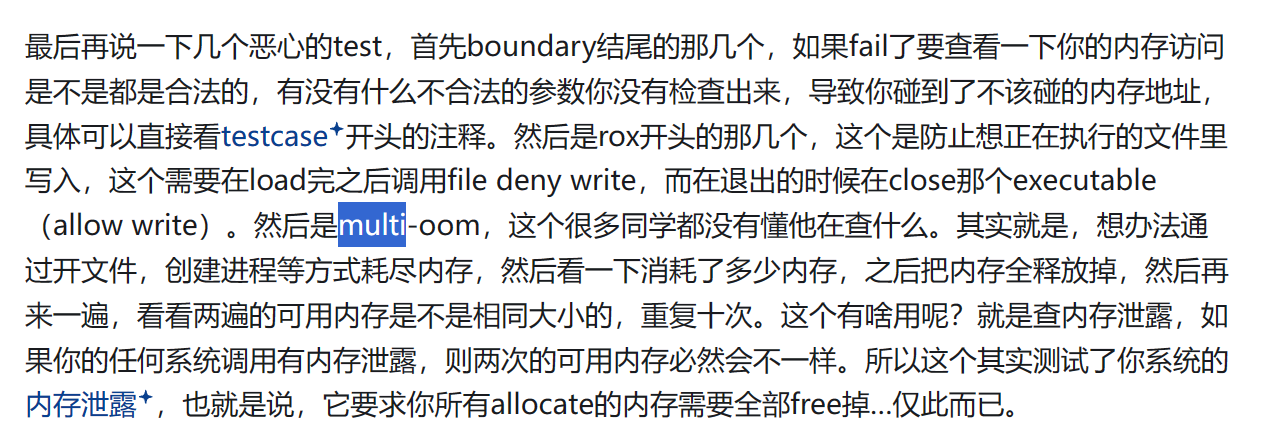
\includegraphics[width=0.6\textwidth]{img6/multioomtip.png}
    \caption{Multi-oom-Tips}
    \label{fig:multi_oom_work}
\end{figure}

所以我感觉,其实只要增大内存,加快运行速度,在 Pintos 设置的 240s 的测试时间内跑完它就好了。

因为我使用的是 Docker 挂载的方法,所以其运行速度和效率远不及内存大的系统。所以我在想,如果放在 Windows 旗下的 WSL 中跑这个测试点呢?
当然,最后我没试,我用了另一个黑科技:

\begin{ans}{}{}

\subsubsection*{使用 \texttt{tmpfs} 挂载}

\texttt{tmpfs} 是内存文件系统,将文件直接挂载到内存中,可以大大提升性能(但受限于内存大小)。

参考资料:Docker 使用 tmpfs 挂载:\href{https://cloud.tencent.com/developer/article/1842268}{\underline{https://cloud.tencent.com/developer/article/1842268}}
\begin{enumerate}
    \item \textbf{启动容器时使用 \texttt{tmpfs} 挂载}:
    \begin{itemize}
        \item docker run --tmpfs /workspace:rw,size=16G -it pintos-container
    \end{itemize}
    \texttt{--tmpfs /workspace:rw,size=16G}:将 \texttt{/workspace} 挂载到内存中,大小为 4GB。
\end{enumerate}

果不其然,在优化了该 Container 的执行效率之后,multi-oom 也通过了。

\end{ans}

愉快提交!接下来好好准备期末,嘿嘿!

\section{附录}

\subsection*{参考资料}

\begin{itemize}
    \item Pintos 单一测试点代码:\href{https://pastebin.com/tFRfywvv}{\underline{https://pastebin.com/tFRfywvv}}
    \item Pintos Lab2:用户程序 User Programs(上):\href{https://blog.csdn.net/Altair_alpha/article/details/126819252}{\underline{https://blog.csdn.net/Altair\_alpha/article/details/126819252}}
    \item Pintos 指导手册:\href{https://pkuflyingpig.gitbook.io/pintos/project-description/lab2-user-programs/suggestions}{\underline{https://pkuflyingpig.gitbook.io/pintos/project-description/lab2-user-programs/suggestions}}
    \item OS实验:pintos project2:\href{https://zhuanlan.zhihu.com/p/382326973}{\underline{https://zhuanlan.zhihu.com/p/382326973}}
    \item 斯坦福大学 Pintos Project1、2 指南+总结:\href{https://zhuanlan.zhihu.com/p/104497182}{\underline{https://zhuanlan.zhihu.com/p/104497182}}
    \item How does thread/process switching work in Pintos?:\href{https://uchicago-cs.github.io/mpcs52030/switch.html}{\underline{https://uchicago-cs.github.io/mpcs52030/switch.html}}
    \item Pintos爆肝实录-User programs:\href{https://zhuanlan.zhihu.com/p/340428650}{\underline{https://zhuanlan.zhihu.com/p/340428650}}
    \item Docker 使用 tmpfs 挂载:\href{https://cloud.tencent.com/developer/article/1842268}{\underline{https://cloud.tencent.com/developer/article/1842268}}
\end{itemize}

\end{document}